\documentclass[12pt,a4paper]{report}

% ============================== PACKAGES ==============================
\usepackage[utf8]{inputenc}
\usepackage[T1]{fontenc}
\usepackage[a4paper,margin=2.7cm,bindingoffset=0.3cm]{geometry}
\usepackage[expansion=false]{microtype}
\usepackage{booktabs}
\usepackage{multirow}
\usepackage{array}
\usepackage{graphicx}
\usepackage{amsmath}
\usepackage{amssymb}
\usepackage{xcolor}
\usepackage{listings}
\usepackage{caption}
\usepackage{subcaption}
\usepackage{enumitem}
\usepackage{setspace}
\usepackage{fancyhdr}
\usepackage{titlesec}
\usepackage[titles]{tocloft}
\usepackage[english]{babel}
\usepackage{csquotes}
\usepackage[round,authoryear]{natbib}
\usepackage[
  hidelinks,
  colorlinks=true,
  linkcolor=blue!55!black,
  urlcolor=blue!55!black,
  citecolor=blue!55!black
]{hyperref}

% ============================== SPACING / LOOK ==============================
\onehalfspacing
\setlength{\parskip}{4pt}
\setlength{\cftbeforechapskip}{8pt}

\titleformat{\chapter}[display]
  {\normalfont\huge\bfseries}{\chaptertitlename\ \thechapter}{16pt}{\Huge}
\titlespacing*{\chapter}{0pt}{0pt}{28pt}

\pagestyle{fancy}
\setlength{\headheight}{14.5pt}
\fancyhf{}
\renewcommand{\headrulewidth}{0.4pt}
\fancyhead[LE,RO]{\thepage}
\fancyhead[RE]{\nouppercase{\leftmark}}
\fancyhead[LO]{\nouppercase{\rightmark}}

% ============================== LISTINGS ==============================
\definecolor{codegray}{rgb}{0.95,0.95,0.95}
\definecolor{codeframe}{rgb}{0.75,0.75,0.75}
\lstdefinestyle{shell}{
  backgroundcolor=\color{codegray},
  basicstyle=\ttfamily\footnotesize,
  breaklines=true,
  frame=single,
  rulecolor=\color{codeframe},
  showstringspaces=false,
  columns=fullflexible,
}
\lstset{style=shell}

% ============================== MISC ==============================
\newcommand{\NOME}{\textsc{nome}}
\newcommand{\ETA}{\textsc{et\`a}}
\newcommand{\DATA}{\textsc{data}}
\newcommand{\LUOGO}{\textsc{luogo\slash indirizzo}}
\renewcommand{\baselinestretch}{1.12}

\begin{document}

% ======================================================================
%                              TITLE PAGE
% ======================================================================
\begin{titlepage}
\begin{center}

\vspace*{0.5cm}
{\large University of Rijeka}\\[0.2cm]
{\large Faculty of Informatics and Digital Technologies}

\vspace{2.2cm}
{\large Dair Sultangazy}

\vspace{2.2cm}
{\Large\bfseries Small Language Models for the De-identification\\[0.2cm] of Italian Health Records}

\vspace{0.6cm}
{\large\itshape Fine-tuning compact open-weight language models to remove\\ personal information from Italian clinical text under a GDPR-motivated,\\ reproducible evaluation protocol}

\vspace{1.8cm}
{\large Master's Thesis}

\vfill

{\large Rijeka, \the\year}

\end{center}
\end{titlepage}

\pagenumbering{roman}

% ======================================================================
%                              ABSTRACT
% ======================================================================
\chapter*{Abstract}
\addcontentsline{toc}{chapter}{Abstract}

Hospitals generate large volumes of free-text clinical narrative that cannot legally leave the institution, or even be used for secondary research inside it, until personally identifying information has been removed. For most languages other than English this is still done by hand or not at all, because the annotated data needed to train a dedicated system rarely exists. This thesis looks at the Italian case specifically, building directly on the 80-note gold-standard benchmark introduced by Miranda et al.~\cite{miranda2025mamma}, who evaluated a panel of instruction-tuned language models in a zero-shot setting and reported a best macro-F1 of 0.620 with a 12-billion-parameter model. Their paper explicitly leaves fine-tuning as future work.

This thesis fills that gap. A 3-billion-parameter model, \texttt{Llama-3.2-3B}, is adapted with low-rank adaptation (LoRA) under 4-bit quantization to perform the redaction task directly -- reading a clinical note and emitting the same note with each personal reference replaced by one of four category tags. Because only 80 annotated notes exist in total, a synthetic data pipeline built on Gemini~2.5~Flash was developed to manufacture additional training material, conditioned on real gold notes so that its narrative style matches the target distribution rather than drifting into generic synthetic text. Under 5-fold cross-validation on the full 80-note set, the resulting model reaches macro-F1 $0.649 \pm 0.073$, exceeding the reference paper's best zero-shot result by 0.029 absolute with a model four times smaller, capable of running on a single 12\,GB consumer GPU. The same pipeline applied to a 1-billion-parameter Gemma-3 model reaches macro-F1 $0.611 \pm 0.109$, essentially matching the 12B zero-shot baseline at twelve times fewer parameters.

Beyond the headline numbers, two findings are, in my view, the more durable contribution of this work. First, the style of synthetic training data matters far more than its volume: an earlier, unconditioned batch of 1000 synthetic notes actively degraded the model to macro-F1 0.18, below every zero-shot baseline in the reference paper, while a few hundred style-anchored notes reversed that collapse entirely. Second, doubling the volume of style-matched synthetic data from roughly 900 to roughly 1800 records did not just raise the mean score, it roughly halved the cross-fold standard deviation, which on an 80-note benchmark is arguably the more practically important effect. The thesis closes with a discussion of where the approach still falls short -- principally on the \NOME{} category, where the small size of the gold set appears to be the binding constraint -- and what a follow-up study with a larger annotated corpus or a BERT-style token-classification baseline would need to look like.

\vspace{1cm}
\noindent\textbf{Keywords:} clinical natural language processing, de-identification, low-resource NLP, parameter-efficient fine-tuning, LoRA, synthetic data, Italian language processing, GDPR

\newpage

% ======================================================================
%                          ACKNOWLEDGMENTS
% ======================================================================
\chapter*{Acknowledgments}
\addcontentsline{toc}{chapter}{Acknowledgments}

I want to thank the authors of the reference study, Miranda et al., for publishing their gold-standard annotations and evaluation code openly -- without a fixed, public benchmark to compare against, none of the comparisons in this thesis would have been possible or meaningful. I am also grateful to the maintainers of the open-weight model families used here (Llama and Gemma) and of the supporting open-source tooling (Hugging Face Transformers, PEFT, TRL, and bitsandbytes), all of which made it possible to run this entire project on a single consumer GPU rather than a research cluster. Finally, thanks to my thesis advisor for pushing back, correctly, on an early single-split result that turned out not to survive cross-validation; that pushback is a large part of why this thesis reports 5-fold CV numbers rather than a single lucky split.

\newpage

% ======================================================================
%                       TABLE OF CONTENTS / FIGURES / TABLES
% ======================================================================
\tableofcontents
\newpage
\listoffigures
\newpage
\listoftables
\newpage

\pagenumbering{arabic}

% ======================================================================
\chapter{Introduction}
\label{ch:intro}
% ======================================================================

\section{Motivation}

An Italian hospital produces, on an ordinary day, hundreds of pages of free-text clinical narrative: discharge letters, radiology reports, nursing notes, referral letters. Almost none of it is written with reuse in mind. A doctor writing ``Rossi Maria, 67 anni, ricoverata il 15/03/2018 presso l'Ospedale San Raffaele di Milano'' is not thinking about the researcher who, two years later, might want to study patterns of hospital readmission across the region. That researcher, under the GDPR and under most national implementations of it, is simply not allowed to see the note in that form. The name, the precise age, the date, and the hospital location together (and sometimes individually) constitute personal data, and personal data cannot be used for secondary research purposes without either explicit consent or an anonymization step that removes the identifying information while, ideally, leaving the clinically useful content intact.

This is not a new problem, and English-language clinical NLP has a fairly mature answer to it. The i2b2/UTHealth shared tasks of 2006 and 2014 established annotated benchmarks and a large research community around automated de-identification of English EHR text, and modern neural sequence taggers routinely report F1 scores above 0.95 on those benchmarks \citep{stubbs2015automated,dernoncourt2017deidentification}. The situation for Italian is very different. There is no equivalent of the i2b2 corpus at scale; annotated clinical text is scarce because hospitals are, understandably, reluctant to share it even for annotation purposes, and the handful of academic efforts that do exist -- the E3C project being the most visible one \citep{magnini2020e3c} -- work with corpora that are one or two orders of magnitude smaller than their English counterparts.

Miranda et al.\ addressed this gap in 2025 by building an 80-note gold-standard benchmark from the CLinkaRT/E3C-derived corpus and evaluating a panel of open-weight instruction-tuned models on it \emph{zero-shot}: no training, just careful prompting \citep{miranda2025mamma}. Their best model, a 12-billion-parameter Gemma-3 variant, reached macro-F1 0.620. That is a genuinely useful number and, at the time it was published, arguably the most rigorous public result for this exact task. But the paper is also explicit about what it did not attempt. Section 6 of Miranda et al.\ states plainly that fine-tuned baselines were out of scope and recommends them as the natural next step. This thesis is, in the most literal sense, an attempt to take that recommendation and see where it leads.

\section{Problem Statement}

The task addressed in this thesis, following the reference paper's formulation exactly so that the two results remain comparable, is \emph{inline redaction}: given a raw Italian clinical note as input, produce the same note as output with every span of personally identifying text replaced by a category placeholder. Four categories are targeted, matching the four for which the reference gold standard has annotations:

\begin{itemize}[nosep]
  \item \NOME{} -- patient and clinician names (\emph{Maria Rossi}, \emph{Dott. Bianchi})
  \item \ETA{} -- age references (\emph{45 anni}, \emph{all'et\`a di 70 anni})
  \item \DATA{} -- dates and temporal expressions (\emph{marzo 2018}, \emph{15/04/2020})
  \item \LUOGO{} -- locations and addresses (\emph{Ospedale San Raffaele, Milano})
\end{itemize}

An example makes the transformation concrete. The input

\begin{quote}
\itshape ``La paziente Maria Rossi, di 67 anni, è stata ricoverata il 15/03/2018 presso l'Ospedale San Raffaele di Milano per dolore toracico.''
\end{quote}

should be rewritten as

\begin{quote}
\itshape ``La paziente [\NOME], di [\ETA], è stata ricoverata il [\DATA] presso [\LUOGO] per dolore toracico.''
\end{quote}

Two constraints shape the rest of this thesis and are worth stating up front, because they rule out several otherwise-obvious approaches. First, the deployment target is a hospital's own hardware, not a cloud API: sending patient text to an external service to redact patient text is close to self-defeating from a privacy standpoint, so the system needs to run entirely on-premise, and realistically on a single consumer- or workstation-grade GPU rather than a multi-node cluster. Second, the amount of labeled Italian clinical text available for training is small -- 80 notes in total, the same 80 used by the reference paper -- which puts this squarely in the regime where naively fine-tuning a large model risks overfitting long before it learns anything general.

\section{Reference Work and Research Gap}

Because this thesis is explicitly built as a head-to-head comparison, it is worth being precise about what exactly is being compared. Miranda et al.\ evaluate five open-weight models --\ \texttt{llama3.2:3b}, \texttt{gemma3:4b}, \texttt{gemma3:12b}, \texttt{mistral:7b}, and \texttt{phi4:14b} -- in a zero-shot, in-context setting: the model is given the note, a natural-language description of the four categories, and asked to redact it directly, with no gradient update ever applied. They use a deterministic, placeholder-counting evaluation metric described in full in Section~\ref{sec:eval-metric}, and their headline number, macro-F1 0.620 for \texttt{gemma3:12b}, is obtained without any task-specific training data at all.

That result is already respectable, but the per-category breakdown in their Table~2 shows an uneven picture. Location and name detection are handled reasonably well by the larger zero-shot models (\LUOGO{} F1 up to 0.88, \NOME{} up to 0.81), but age detection is consistently poor -- their best \ETA{} score across all five models is 0.41, and their best individual model, \texttt{gemma3:12b}, scores only 0.14 on that category specifically, apparently because age mentions in Italian clinical prose (\emph{``vent'anni di ipertensione''}, a twenty-year history of hypertension, not a twenty-year-old patient) are easy for a general-purpose model to confuse with durations or unrelated numeric spans. Date detection sits in between, topping out at 0.65.

This unevenness is the research gap this thesis targets directly. If age-format ambiguity is a knowledge gap rather than a capacity gap -- if the model simply hasn't seen enough labeled examples of how Italian clinical prose expresses age, rather than being fundamentally too small to represent the concept -- then fine-tuning on even a modest number of correctly labeled examples should close much of it, and should do so with a model considerably smaller than 12B parameters. That is the hypothesis this thesis sets out to test.

\section{Research Questions and Objectives}

Three questions organize the experimental work that follows.

\textbf{RQ1.} Can a fine-tuned model with substantially fewer parameters than the strongest zero-shot baseline (\texttt{gemma3:12b}, 12B parameters) match or exceed it on the same 80-note benchmark, under a cross-validation protocol rather than a single train/test split?

\textbf{RQ2.} Given that only 80 gold-annotated notes exist, what role does synthetic training data play, and does its \emph{style} -- how closely it mimics the surface form, vocabulary, and entity distribution of real Italian clinical notes -- matter more or less than its raw volume?

\textbf{RQ3.} Does the answer to RQ1 depend on model scale within the small-model regime -- that is, does a 1B-parameter model fine-tuned the same way behave qualitatively like the 3B model, or does capacity become a binding constraint below some threshold?

The corresponding objectives were: (i) build a two-phase training pipeline -- continual pre-training for domain vocabulary followed by supervised fine-tuning for the redaction task -- on top of an open-weight 3B model under LoRA and 4-bit quantization; (ii) design and validate a synthetic data generation pipeline that could be audited for style match against the gold notes, rather than trusting a generic prompt to produce clinically plausible text; (iii) evaluate everything under the reference paper's exact metric and, additionally, under 5-fold cross-validation, since an 80-note test set is small enough that a single split can be badly misleading; and (iv) repeat the full pipeline on a second, smaller base model to see whether the result generalizes across architecture and scale.

\section{Contributions}

This thesis makes the following contributions.

\textbf{A fine-tuned model that beats the strongest zero-shot baseline under cross-validation.} \texttt{Llama-3.2-3B}, fine-tuned with LoRA in 4-bit precision, reaches macro-F1 $0.649 \pm 0.073$ under 5-fold CV on the full 80-note gold standard, against the reference paper's best zero-shot result of 0.620 -- a model roughly four times smaller, running comfortably within 12\,GB of GPU memory.

\textbf{A cross-architecture replication at 1B parameters.} The identical pipeline applied to \texttt{gemma-3-1b-it} reaches macro-F1 $0.611 \pm 0.109$, within statistical noise of the 12B zero-shot baseline at twelve times fewer parameters, though with visibly higher fold-to-fold variance than the 3B model.

\textbf{A style-anchored synthetic data pipeline for a genuinely low-resource setting.} Rather than prompting a large model for generic synthetic clinical notes, the pipeline conditions generation on real gold notes as few-shot style anchors, enforces a schema-constrained output format, and validates every generated case against a set of structural and entity-consistency checks before it is admitted to the training set. The full pipeline, at roughly \$15 in API cost, produced around 1800 usable synthetic notes.

\textbf{An empirical demonstration that synthetic-data style transfer dominates volume.} A controlled comparison shows that 1000 synthetic notes generated without style anchoring actively harm the model (macro-F1 0.18, below every zero-shot baseline reported by Miranda et al.), while a few hundred style-anchored notes reverse the collapse and push performance well past the zero-shot ceiling. This finding, more than the specific F1 numbers, is the part of this thesis I would expect to generalize to other low-resource clinical NLP settings.

\textbf{A documented and reproducible negative result.} An attempt to fit a 4-billion-parameter Gemma-3 variant on the same 12\,GB GPU failed at the loss-computation step due to the model's unusually large 262K-token vocabulary, even after aggressive memory-saving measures. This is reported in Section~\ref{sec:gemma4b-oom} not as a footnote but as a genuine finding about which small-model architectures are actually deployable under consumer hardware constraints.

\section{Thesis Structure}

The remainder of this thesis is organized as follows. Chapter~\ref{ch:background} introduces the technical background needed to follow the rest of the thesis without prior exposure to transformer-based language modeling: the transformer architecture itself, the shift from pretraining to instruction-tuned models, de-identification as a variant of named entity recognition, parameter-efficient fine-tuning and specifically LoRA, quantization and QLoRA, and the legal framing that motivates the whole exercise. Chapter~\ref{ch:related} reviews the closest prior work in more depth, organized around five threads: classical and neural clinical de-identification, Italian and multilingual clinical NLP resources, parameter-efficient fine-tuning of LLMs, synthetic data generation for low-resource fine-tuning, and LLM-based text anonymization more broadly. Chapter~\ref{ch:data} describes the dataset in detail, including the design and validation of the synthetic data pipeline. Chapter~\ref{ch:method} describes the training pipeline, model configuration, and evaluation protocol. Chapter~\ref{ch:results} presents the experimental results, including the iteration history that led to the final configuration, the main cross-validation results, and the cross-architecture comparison. Chapter~\ref{ch:discussion} interprets those results and discusses why fine-tuning helps where it helps and not where it doesn't. Chapter~\ref{ch:limitations} lays out the limitations of the study and directions for follow-up work, and Chapter~\ref{ch:conclusion} concludes.

% ======================================================================
\chapter{Background}
\label{ch:background}
% ======================================================================

This chapter introduces the concepts that the rest of the thesis relies on. Readers already comfortable with transformer language models and parameter-efficient fine-tuning can skip to Chapter~\ref{ch:related} without losing continuity; the point of this chapter is to make the methodology chapter legible to a reader coming from a clinical-informatics or general software-engineering background rather than an NLP research background.

\section{Transformer Language Models}

Almost every model discussed in this thesis is a decoder-only transformer, a neural network architecture built entirely out of self-attention layers rather than the recurrent or convolutional layers that dominated NLP before 2017 \citep{vaswani2017attention}. At a high level, a transformer language model represents a piece of text as a sequence of tokens -- units roughly the size of a short word or a word fragment -- and, at each layer, lets every token attend to every other token in the sequence, computing a weighted combination of their representations. Stacking many such layers produces representations that encode increasingly abstract information: early layers tend to capture local syntax, later layers more contextual and semantic information. The key practical property that makes transformers attractive for this thesis is that a single architecture, trained self-supervised on next-token prediction over a large text corpus, transfers reasonably well to a wide range of downstream tasks with comparatively little task-specific data -- which matters enormously given how little labeled Italian clinical text exists.

\texttt{BERT} \citep{devlin2019bert} popularized a closely related but architecturally distinct idea -- bidirectional, encoder-only pretraining for representation learning, typically paired with a lightweight task-specific head for classification or tagging. It is worth flagging this distinction early, because the ``obvious'' architecture for a de-identification system is arguably a BERT-style token classifier rather than a decoder-only generative model, and Section~\ref{sec:limitations-bert} returns to why this thesis does not use one, despite BERT-style systems being the dominant paradigm in the English de-identification literature reviewed in Chapter~\ref{ch:related}.

\section{From Pretraining to Instruction-Tuned Models}

The models used in this thesis -- \texttt{Llama-3.2-3B} and \texttt{Gemma-3} -- are decoder-only, autoregressive models: given a sequence of tokens, they predict a probability distribution over the next token, one token at a time. Pretraining on large, mostly unlabeled text corpora gives these models broad linguistic and world knowledge but no particular tendency to follow instructions or behave like a well-mannered assistant; a raw pretrained model asked to redact a clinical note is as likely to continue the note as to redact it. Instruction tuning -- further training on curated (instruction, response) pairs, sometimes followed by preference optimization -- is what turns a base language model into something that reliably follows a task description. The models used as zero-shot baselines by Miranda et al., and the base checkpoints fine-tuned further in this thesis, are all instruction-tuned variants (denoted \texttt{-it} for Gemma and implicit for the Llama-3.2-Instruct family).

This distinction matters for two reasons that recur throughout the thesis. First, it is the instruction-tuned checkpoint's chat template -- the specific sequence of special tokens that demarcate system, user, and assistant turns -- that has to be respected exactly during fine-tuning, or the model's learned turn-taking behavior breaks (Section~\ref{sec:chat-template}). Second, instruction tuning is itself a form of fine-tuning, which means the zero-shot baselines in the reference paper are not really ``untrained'' in an absolute sense -- they already reflect substantial task-agnostic supervision. The comparison in this thesis is therefore more precisely stated as: does \emph{additional}, task-specific fine-tuning on top of an already instruction-tuned checkpoint outperform prompting that same family of checkpoints zero-shot on this particular task.

\section{De-identification as Named Entity Recognition}

De-identification and named entity recognition (NER) are, formally, close to the same problem. NER assigns a category label to spans of text corresponding to entities of interest -- people, organizations, locations, dates -- and de-identification narrows that label set to categories considered personally identifying and adds a downstream redaction or substitution step. The English clinical NLP literature has largely treated de-identification exactly this way: as sequence labeling, typically with a BIO or BILOU tagging scheme over subword tokens, trained end-to-end on annotated corpora such as i2b2/UTHealth \citep{stubbs2015automated,dernoncourt2017deidentification}.

This thesis, and the reference paper it builds on, instead frame de-identification as a sequence-to-sequence \emph{redaction} task: the model reads the full note and writes out a new version of it with identifying spans replaced by placeholder tags, rather than emitting a list of (span, label) pairs. This has a practical advantage for evaluation with generative LLMs, since it sidesteps the brittle problem of aligning model-generated entity boundaries with gold character offsets, and a practical disadvantage in that it gives up some of the precision that comes from explicit span-level supervision. Section~\ref{sec:eval-metric} describes the evaluation metric that makes redaction-style output scoreable at all, and Section~\ref{sec:limitations-bert} discusses what would change if the task were reframed as token classification instead.

\section{Parameter-Efficient Fine-Tuning and LoRA}

Fully fine-tuning a multi-billion-parameter model -- updating every weight -- is expensive in both compute and, critically for this thesis, GPU memory, since the optimizer state for adaptive methods like Adam requires storing multiple auxiliary tensors per parameter. Parameter-efficient fine-tuning (PEFT) methods instead freeze the pretrained weights and introduce a much smaller number of trainable parameters, updating only those \citep{xu2024peft}. Low-Rank Adaptation, or LoRA \citep{hu2021lora}, is the specific PEFT method used throughout this thesis. The idea is to represent the weight \emph{update} for a given linear layer, rather than the weight itself, as a product of two low-rank matrices $A \in \mathbb{R}^{d \times r}$ and $B \in \mathbb{R}^{r \times k}$, where $r$ (the rank) is chosen to be far smaller than the layer's original dimensions $d$ and $k$. The effective forward pass becomes

\[
h = W_0 x + \Delta W x = W_0 x + BAx,
\]

where $W_0$ is the frozen pretrained weight matrix. Only $A$ and $B$ are trained; $W_0$ never changes. Because $r \ll \min(d,k)$, the number of trainable parameters introduced by a LoRA adapter is a tiny fraction of the base model's total parameter count -- in this thesis, roughly 1.7\% (Section~\ref{sec:model-config}). Hu et al.\ show that this restriction to a low-rank update does not meaningfully hurt task performance relative to full fine-tuning across a range of models and tasks, and has the practical side benefit of producing a small, portable adapter file (tens of megabytes) rather than a full copy of the model for every fine-tuned variant.

\section{Quantization and QLoRA}

Quantization reduces the numerical precision used to store model weights -- for example, from 16-bit floating point down to 4-bit integers -- trading a small amount of numerical fidelity for a large reduction in memory footprint. QLoRA \citep{dettmers2023qlora} combines this idea with LoRA: the frozen base model is stored in 4-bit precision using a specialized data type, 4-bit NormalFloat (NF4), chosen to be information-theoretically well matched to the roughly normal distribution of pretrained transformer weights, while the LoRA adapter matrices themselves are still trained in higher precision (bfloat16 in this thesis) and gradients are backpropagated through the quantized base weights without ever fully dequantizing them into memory. QLoRA additionally introduces double quantization, which quantizes the quantization constants themselves for a further, smaller memory saving, and paged optimizers that spill optimizer state to CPU memory during transient GPU memory spikes rather than causing an out-of-memory crash. This combination is what makes it possible to fine-tune a 3B-parameter model, end to end, on a single 12\,GB consumer GPU, and it is the exact configuration used for both models trained in this thesis (Section~\ref{sec:model-config}).

\section{Evaluating De-identification Systems}
\label{sec:eval-metric}

De-identification systems are conventionally evaluated with precision, recall, and F1 computed over predicted spans against gold-annotated spans, typically requiring exact or near-exact boundary overlap. That standard is difficult to apply directly to a generative redaction model, whose output is free text rather than a structured list of spans with character offsets, and whose placeholder insertion may not align perfectly with the original span boundaries even when it captures the right entity.

The reference paper -- and, for direct comparability, this thesis -- instead uses a deterministic \emph{placeholder-counting} metric. For each PII category $T$ (e.g.\ \NOME), and for a given note, let $g_T$ be the number of gold entities of type $T$, and let $c_T$ be the number of $\texttt{[}T\texttt{]}$ placeholder tags the model actually emitted in its redacted output. False negatives are counted as the number of gold entity \emph{surface strings} of type $T$ that are still literally present, uncensored, somewhere in the model's output:

\[
\text{FN}_T = |\{ e \in \text{gold entities of type } T : e \text{ appears verbatim in model output} \}|.
\]

True positives are then $\text{TP}_T = g_T - \text{FN}_T$, and false positives are the excess of emitted placeholders over gold entities, floored at zero: $\text{FP}_T = \max(0,\ c_T - g_T)$. Precision, recall, and F1 are computed from these counts in the usual way, and the headline metric, macro-F1, is the unweighted mean of the four per-category F1 scores. This metric is deliberately forgiving of imperfect boundary placement -- it does not check that the placeholder appears exactly where the entity used to be, only that the entity is gone from the text and that the placeholder count is not wildly inflated -- which suits a generative model that was never trained to output character-level span boundaries in the first place. It also means the metric can be fooled by a degenerate strategy of replacing everything with every tag, which is why the false-positive term matters: an over-eager model that redacts everything gets punished on precision for each category it over-tags.

\section{GDPR, Anonymization, and the Legal Framing}

The GDPR (Regulation (EU) 2016/679) distinguishes between \emph{anonymized} data, from which no individual can reasonably be re-identified and which therefore falls outside the regulation's scope entirely, and \emph{pseudonymized} data, where identifying information has been replaced by artificial identifiers but a mapping back to the original individual still exists somewhere and the data therefore remains personal data under the law. The placeholder-tag substitution used in this thesis and in the reference paper -- replacing a name with the literal string \texttt{[\NOME{}]} rather than with a consistent surrogate name -- sits closer to anonymization than pseudonymization in intent, in that no reversible mapping is preserved, though whether a given redacted note meets the GDPR's actual bar for anonymization (which requires considering re-identification risk from context, not just from the removed spans themselves) is a legal determination this thesis does not attempt to make. What this thesis evaluates is a narrower, well-defined technical question -- how completely and how precisely a system removes four specific categories of identifying spans -- which is a necessary but not sufficient condition for GDPR-compliant anonymization in the full legal sense. Recent NLP work on LLM-based anonymization has begun to treat privacy and downstream utility as a joint optimization problem rather than pure span removal \citep{yang2025rupta}; Section~\ref{sec:future-work} returns to how that line of work might extend the approach taken here.

% ======================================================================
\chapter{Related Work}
\label{ch:related}
% ======================================================================

This chapter reviews the prior work most directly relevant to this thesis, organized into five threads: the evolution of clinical de-identification from rule-based to neural systems, Italian and multilingual clinical NLP resources, parameter-efficient fine-tuning of large language models, synthetic data generation for low-resource fine-tuning, and LLM-based text anonymization as a broader research area. The chapter closes by positioning this thesis relative to all five.

\section{Clinical De-identification: From Rules to Neural Sequence Labeling}

Automated clinical de-identification has a longer history in English-language NLP than the framing of this thesis might suggest. Early systems relied heavily on hand-written rules and dictionaries -- lists of common names, regular expressions for date and phone-number formats -- and while such systems could achieve high precision on the patterns they were built for, they generalized poorly to novel name variants, misspellings, or institution-specific formatting conventions. The i2b2/UTHealth shared tasks, first run in 2006 and revisited in 2014 with a large, longitudinal corpus of 1,304 records covering 296 patients and over 28,000 annotated PHI instances, gave the field a common benchmark and pushed it decisively toward statistical and later neural methods \citep{stubbs2015automated}. By the time Dernoncourt et al.\ published the first artificial-neural-network-based de-identification system in 2017, framed as token-level sequence labeling with a bidirectional LSTM and requiring no hand-crafted features, the field had already largely moved past rule-based approaches \citep{dernoncourt2017deidentification}. Subsequent transformer-based systems, typically fine-tuned BERT variants performing BIO tagging, have pushed reported F1 on the 2014 i2b2 benchmark well above 0.95, a threshold generally treated in the literature as comparable to manual annotation quality.

Two things are worth noting about this trajectory for the purposes of this thesis. First, essentially all of this progress happened within a supervised sequence-labeling paradigm, trained on corpora that are, in absolute terms, enormous compared to what exists for Italian -- the i2b2 2014 corpus alone contains more than 1,300 documents, against 80 for the Italian benchmark used here. Second, none of it involved framing the task as free-text generation the way this thesis does; the redaction-as-generation framing used here and by Miranda et al.\ is a comparatively recent development, made practical only by instruction-tuned generative LLMs capable of following a redaction instruction directly.

\section{Italian and Multilingual Clinical NLP Resources}

Italian clinical NLP suffers from the resource scarcity common to most languages other than English, but not from a complete absence of effort. The European Clinical Case Corpus (E3C) project assembled and annotated clinical case narratives across five languages -- Italian, English, French, Spanish, and Basque -- with a two-level annotation scheme covering clinical entities (pathologies, procedures, anatomical terms, tied to SNOMED-CT and ICD-10 taxonomies) and temporal/factuality information \citep{magnini2020e3c}. E3C was not built specifically as a de-identification corpus, but its Italian clinical-case narratives, and the annotation infrastructure built around them, form the basis of the CLinkaRT-derived gold standard that both Miranda et al.\ and this thesis use.

The reference work of this thesis, Miranda et al.'s ``Mamma Mia! Where's My Name?'' \citep{miranda2025mamma}, is to my knowledge the most recent published benchmark specifically for Italian clinical de-identification, and the first to evaluate open-weight LLMs zero-shot on the task rather than training a dedicated tagger. Their 80-note gold standard, four-category annotation scheme (\NOME, \ETA, \DATA, \LUOGO), and deterministic placeholder-counting metric are all adopted unchanged in this thesis specifically so that the results reported here are comparable, table for table, with theirs. Their paper's own related-work discussion notes the absence of a fine-tuned baseline as a limitation; this thesis is best read as a direct response to that specific gap, using their own benchmark as the test bed.

\section{Parameter-Efficient Fine-Tuning of Large Language Models}

The practical feasibility of this thesis rests on parameter-efficient fine-tuning research from the last several years. LoRA \citep{hu2021lora} established that injecting trainable low-rank update matrices into a frozen pretrained model's linear layers can match full fine-tuning quality while training a tiny fraction of the parameters, with no added inference latency once the adapter is merged. QLoRA \citep{dettmers2023qlora} extended this by showing that the frozen base model itself can be stored in 4-bit precision -- using the NF4 data type and double quantization described in Section~\ref{ch:background} -- without meaningfully degrading the quality of the resulting fine-tuned model, reporting that their best 4-bit fine-tuned model reached 99.3\% of ChatGPT's performance on a conversational benchmark after 24 hours of training on a single GPU. A broader survey of the PEFT landscape by Xu et al.\ situates LoRA within a larger family of approaches -- additive methods like adapters and prompt tuning, selective methods that fine-tune only a subset of existing parameters, and reparameterization methods like LoRA itself -- and notes that reparameterization methods have become the dominant choice for consumer-hardware fine-tuning specifically because, unlike adapters, they introduce zero additional inference-time computation once merged into the base weights \citep{xu2024peft}. This thesis uses exactly the QLoRA configuration -- LoRA adapters over a 4-bit NF4-quantized base model -- for both models trained, and Section~\ref{sec:model-config} reports the specific rank, target modules, and quantization settings used.

\section{Synthetic Data Generation for Low-Resource Fine-Tuning}

Given that the Italian gold standard used here contains only 80 notes, and that a meaningful held-out test set further shrinks the usable training pool, some form of data augmentation is close to unavoidable. A growing body of work uses large language models themselves to generate synthetic training data for smaller, task-specific models, sometimes framed explicitly as knowledge distillation from a larger teacher model to a smaller student. Woo et al.\ demonstrate this pattern in a clinical context: using a 70B-parameter Llama model to generate synthetic question-answer training pairs, they fine-tune an 8B-parameter model that in some cases outperforms its own 70B teacher on the target extraction task, while running at a fraction of the inference cost \citep{woo2024syntheticdistillation}. More broadly, recent surveys of synthetic data generation in biomedical NLP report that LLM-prompted generation is now the dominant method for producing synthetic training data in this space, ahead of fine-tuning-based generation and specialized generative models, precisely because it requires no additional training infrastructure of its own.

What this literature does not, in general, emphasize is the risk this thesis found to be dominant in practice: that synthetic data whose surface style does not match the target distribution can actively harm a downstream model rather than merely fail to help it. Section~\ref{sec:no-gold-control} reports a controlled experiment in which training exclusively on unconditioned synthetic notes drove macro-F1 to 0.18, below every zero-shot baseline in the reference paper -- worse, in other words, than doing nothing. This result motivated the style-anchored generation approach described in Chapter~\ref{ch:data}, in which every synthetic note is generated with real gold notes embedded as few-shot exemplars specifically to constrain surface style, rather than relying on a generic system prompt describing the target domain in the abstract.

\section{LLM-Based Text Anonymization}

A separate but related line of work treats LLMs not as the system being protected against re-identification, but as the anonymization tool itself, and increasingly frames anonymization as a joint optimization between privacy and utility rather than pure entity removal. Yang et al.\ propose a framework with separate LLM-based privacy and utility evaluators coordinating an anonymization component, arguing that na\"ive span removal can both under-protect against a sufficiently capable re-identifying adversary and over-damage the residual usefulness of the text for downstream tasks \citep{yang2025rupta}. This thesis's task is narrower and more constrained than that framing -- four fixed categories, a fixed deterministic metric, direct comparability with a specific prior benchmark -- but the broader anonymization literature is a useful pointer to what a production-grade successor to this system would need to add: an explicit accounting of residual re-identification risk from the \emph{combination} of remaining context, not just from the four tagged categories in isolation, which the placeholder-counting metric used here does not capture at all.

\section{Italian-Native Language Models}

Nearly all of the models evaluated in this thesis and in the reference paper -- Llama, Gemma, Mistral, Phi -- are trained predominantly on English-dominant multilingual corpora and adapted to Italian largely through the presence of Italian text in that broader pretraining mixture, rather than through Italian-first pretraining. A more recent development, arriving after most of the experimental work in this thesis was designed, is Minerva, the first family of LLMs pretrained from scratch with Italian as a first-class language rather than an afterthought, released in sizes from 350M to 7B parameters and trained on a roughly balanced mixture of Italian and English tokens plus code \citep{orlando2024minerva}. The reference paper itself flags an Italian-native base model as a promising direction for future work, and this thesis inherits that suggestion largely unexamined: whether continual pretraining plus LoRA fine-tuning on a Minerva checkpoint would close more of the remaining \NOME{} gap than the Llama-based pipeline used here is, at the time of writing, untested, and is discussed further as future work in Section~\ref{sec:future-work}.

\section{Positioning of This Work}

Table~\ref{tab:related-positioning} summarizes where this thesis sits relative to the threads reviewed above. Relative to the classical clinical de-identification literature, this thesis works with two orders of magnitude less annotated data and a generative rather than sequence-labeling formulation. Relative to the reference paper, it adds exactly the fine-tuned baseline that paper identifies as missing, under an evaluation protocol (5-fold CV) that is strictly more demanding than the paper's own single-split zero-shot evaluation. Relative to the PEFT and synthetic-data literature, it is not methodologically novel in isolation -- LoRA, QLoRA, and LLM-prompted synthetic data generation are all established techniques -- but the specific combination, applied to an extremely small (80-note) real-world clinical corpus in a genuinely low-resource language, and the explicit ablation of synthetic-data \emph{style} against synthetic-data \emph{volume}, is, to my knowledge, not something the existing literature has reported for this task or this language.

\begin{table}[htbp]
\centering
\caption{Positioning of this thesis relative to the closest prior work.}
\label{tab:related-positioning}
\begin{tabular}{p{3.6cm}p{5.6cm}p{5.6cm}}
\toprule
Thread & Prior work & This thesis \\
\midrule
Clinical de-id (English) & Large annotated corpora (1000s of notes); sequence labeling \citep{stubbs2015automated,dernoncourt2017deidentification} & 80 notes; generative redaction \\
Italian clinical de-id & Zero-shot LLM prompting, no fine-tuning \citep{miranda2025mamma} & Adds the fine-tuned baseline explicitly left as future work \\
PEFT & LoRA/QLoRA as general-purpose methods \citep{hu2021lora,dettmers2023qlora} & Applied specifically to an 80-note clinical benchmark \\
Synthetic data & Volume-oriented LLM-prompted generation \citep{woo2024syntheticdistillation} & Explicit style-vs-volume ablation; style-anchored generation \\
LLM anonymization & Privacy--utility joint optimization \citep{yang2025rupta} & Narrower 4-category task, fixed deterministic metric \\
\bottomrule
\end{tabular}
\end{table}

% ======================================================================
\chapter{Dataset and Data Engineering}
\label{ch:data}
% ======================================================================

If there is a single thread that ties the results in this thesis together, it is that the data, not the model or the training recipe, turned out to be the decisive variable. This chapter describes the gold standard inherited from the reference paper, the entity categories in detail, and -- at greater length, because it is where most of the actual engineering effort went -- the synthetic data pipeline built to compensate for the small size of the gold set.

\section{The Gold Standard}

The gold standard used throughout this thesis, \texttt{gold\_standard\_80.json}, is the identical 80-note benchmark released by Miranda et al., derived from the CLinkaRT/E3C Italian clinical corpus. Each record consists of a free-text clinical narrative -- typically a few hundred to a few thousand characters, describing a patient's presentation, history, and course of treatment in the register of a hospital discharge or case summary -- together with a list of manually annotated entities, each tagged with its category and exact surface form. Table~\ref{tab:entity-counts} gives the entity counts across the full 80-note set.

\begin{table}[htbp]
\centering
\caption{Entity counts in the 80-note gold standard.}
\label{tab:entity-counts}
\begin{tabular}{lrl}
\toprule
Category & Count & Notes \\
\midrule
\NOME{} & 46 & Many notes contain zero name mentions \\
\ETA{} & 89 & \\
\DATA{} & 78 & \\
\LUOGO{} & 142 & Most frequent category \\
\midrule
Total & 355 & \\
\bottomrule
\end{tabular}
\end{table}

The distribution in Table~\ref{tab:entity-counts} is not balanced, and the imbalance turned out to matter a great deal for the synthetic data design described below. \LUOGO{} is by far the most frequent category, while \NOME{} is the rarest -- many notes never mention a patient or clinician by name at all, referring to ``la paziente'' or ``il soggetto'' instead, which is itself a reasonable stylistic norm for case-report-style clinical writing and not an annotation artifact. This asymmetry is easy to overlook when generating synthetic training data with a generic prompt, and Section~\ref{sec:nome-overrep} describes what happened when it was overlooked.

Because keeping the same 80-note evaluation set as the reference paper was a hard requirement for comparability, no additional real annotation was performed. All augmentation had to come from elsewhere.

\section{Entity Category Definitions}

Table~\ref{tab:category-examples} restates the four categories with representative examples, adapted from the reference paper's annotation guidelines and cross-checked against the gold standard itself. A recurring theme in these examples, and one of the harder aspects of the task, is that Italian clinical prose frequently expresses age and duration using overlapping surface forms -- ``da 20 anni'' can mean ``for 20 years'' (a duration, not tagged) or, in a different sentence, be adjacent to an actual age reference -- which is precisely the kind of ambiguity that a zero-shot model, lacking task-specific examples, tends to resolve incorrectly.

\begin{table}[htbp]
\centering
\caption{PII category definitions and examples.}
\label{tab:category-examples}
\begin{tabular}{p{2.6cm}p{5.2cm}p{5.6cm}}
\toprule
Category & Description & Examples \\
\midrule
\NOME{} & Patient or clinician personal names & \emph{Maria Rossi}, \emph{Dott. Bianchi} \\
\ETA{} & Age references, in years & \emph{45 anni}, \emph{all'et\`a di 70 anni} \\
\DATA{} & Dates, including partial dates & \emph{marzo 2018}, \emph{15/04/2020}, \emph{2017} \\
\LUOGO{} & Locations, addresses, institutions & \emph{Ospedale San Raffaele, Milano} \\
\bottomrule
\end{tabular}
\end{table}

\section{The Case for Synthetic Data}

Eighty notes, split five ways for cross-validation, leaves 64 notes per training fold. That is not enough to fine-tune a 3-billion-parameter model without either drastically restricting what changes (which LoRA already does, at the parameter level) or accepting a very real risk of memorizing the training folds rather than learning generalizable redaction behavior -- a risk that is easy to underestimate until it shows up as a suspiciously good single-split score that collapses under cross-validation, which is more or less exactly what happened during an earlier iteration of this project (Section~\ref{sec:iteration-timeline}). Some form of additional training signal was necessary, and given the total absence of a larger existing Italian clinical corpus with matching annotations, the practical options were essentially: (a) find or construct additional annotated real data, which was infeasible for this thesis given data-access constraints on real clinical text, or (b) generate synthetic data with an existing LLM. This thesis takes the second path, using Gemini~2.5~Flash as the generator.

\section{Style-Anchored Synthetic Generation}
\label{sec:style-anchoring}

An early version of the synthetic data used in this project -- a batch of 1000 generic synthetic clinical notes produced with a straightforward prompt describing the task in the abstract, without reference to real examples -- turned out, on later inspection, to be stylistically quite different from the gold notes: entity density, sentence structure, and narrative register all diverged noticeably. Training on that batch alone, discussed in full in Section~\ref{sec:no-gold-control}, produced a model that performed \emph{worse} than every zero-shot baseline in the reference paper. That failure is what motivated the redesigned pipeline described here.

The redesigned generator, implemented in \texttt{generate\_synthetic\_v2.py} and its name-free counterpart \texttt{generate\_noname.py}, embeds three real gold notes directly into every generation prompt as few-shot style anchors -- one short, one medium-length, one long, chosen to span the range of note lengths actually present in the gold set. Beyond the style anchors, each generation batch rotates a set of diversity controls (medical specialty, patient gender, age range, and target entity density) so that the resulting corpus does not collapse into near-duplicate cases, and the generation call constrains Gemini's output to a fixed JSON schema via the API's \texttt{response\_schema} parameter, which all but eliminates the malformed-JSON failures that a free-text generation prompt would otherwise produce at scale.

Several additional constraints were added to the prompt after inspecting early outputs: third-person past-tense narration (matching the register of the gold notes, which read like retrospective case summaries rather than live clinical documentation); realistic Italian medical vocabulary density; genuine Italian names, cities, and hospital names rather than obviously placeholder-style ones; a deliberate mix of date formats (\emph{``marzo 2018''}, \emph{``15/04/2020''}, bare years like \emph{``2017''}) rather than a single canonical format, since the gold notes themselves mix formats; and, where a patient name is present at all, repetition of that name three to six times across the note via anaphora, which is how the gold notes typically refer back to a named patient.

Every generated case is then passed through a validation gate before being admitted to the training pool. A case is accepted only if every entity listed in its \texttt{entities} field appears as a literal substring in the generated \texttt{text}; no entity's surface text appears anywhere in the corresponding \texttt{redacted\_text}, which would indicate an incomplete redaction; every entity category actually present in the case has a matching \texttt{[TYPE]} placeholder somewhere in \texttt{redacted\_text}; at least two valid entities are present, to filter out degenerate near-empty cases; and the note length falls within a plausible range (1000--4000 characters, chosen to match the observed length distribution of the gold notes). Roughly 77\% of generated with-name cases and 71\% of generated name-free cases passed this gate on the first attempt, the lower name-free pass rate reflecting the additional, stricter constraint that no \NOME{} entity be present at all. Manual inspection of twenty randomly sampled accepted cases found their surface style effectively indistinguishable from gold notes to a non-expert reader, and their length distribution (1021--3678 characters, mean 2250) closely tracked the gold set's own range (roughly 1500--3500 characters).

\section{The \NOME{} Over-Representation Problem}
\label{sec:nome-overrep}

An early version of the style-anchored pipeline (before the name-free variant existed) produced 624 with-name synthetic cases, \texttt{synthetic\_v2\_1000.json}, and training on that batch alone -- alongside the gold notes -- yielded a respectable overall macro-F1 of 0.635 on a single held-out split, but a strikingly weak \NOME{} score specifically: F1 0.36, with precision only 0.29, meaning the model was over-tagging names far more often than it was correctly recalling them. Diagnosing this required going back to the entity statistics rather than trusting the aggregate score. The gold standard, as Table~\ref{tab:entity-counts} shows, contains 46 \NOME{} entities across 80 notes -- an average of 0.58 name mentions per note, and many notes with zero. The 624-case synthetic batch, by contrast, contained 1485 \NOME{} entities, an average of 2.38 per case, because \emph{every} synthetic case included a named patient by construction. That is roughly a four-fold over-representation of names relative to the target distribution, and the model, quite reasonably given what it was shown, learned that names are far more common in clinical text than they actually are in this corpus, and over-redacted accordingly.

The fix was to generate an explicitly name-free complement to the with-name synthetic set. \texttt{generate\_noname.py} runs the same style-anchored pipeline but instructs the generator to refer to the patient only through anonymous descriptors (\emph{``la paziente''}, \emph{``l'uomo''}, \emph{``il soggetto''}) and adds an explicit rejection rule to the validation gate: any case containing a \NOME{} entity is discarded outright. Adding 254 of these name-free cases to the training mix moved \NOME{} F1 from 0.36 to 0.50 on the same held-out split (precision from 0.29 to 0.50), with no measurable degradation in the other three categories -- a clean confirmation that the problem really had been entity-distribution mismatch rather than, say, insufficient overall training volume.

\section{Final Training Data Composition}

The final training configuration used for the headline result in this thesis, referred to throughout as \emph{v4}, combines four sources per cross-validation fold, summarized in Table~\ref{tab:data-composition-thesis} and shown graphically in Figure~\ref{fig:data-composition}.

\begin{table}[htbp]
\centering
\caption{Composition of the v4 training set (per fold).}
\label{tab:data-composition-thesis}
\begin{tabular}{p{3.9cm}rp{7.2cm}}
\toprule
Source & Records & Role \\
\midrule
Gemini synthetic, with names & 1201 & Style-anchored generated notes with a named patient (Section~\ref{sec:style-anchoring}) \\
Gemini synthetic, name-free & 475 & Style-anchored generated notes with no \NOME{} entity, for distribution rebalancing (Section~\ref{sec:nome-overrep}) \\
Gold standard (train fold) & $64 \times 5 = 320$ & 5$\times$ oversampled to give it comparable weight against the larger synthetic pool \\
CRF negative samples & 80 & No-PII text; teaches ``not every note needs redaction'' \\
\midrule
\textbf{Total per fold} & \textbf{2076} & \\
\bottomrule
\end{tabular}
\end{table}

\begin{figure}[htbp]
\centering
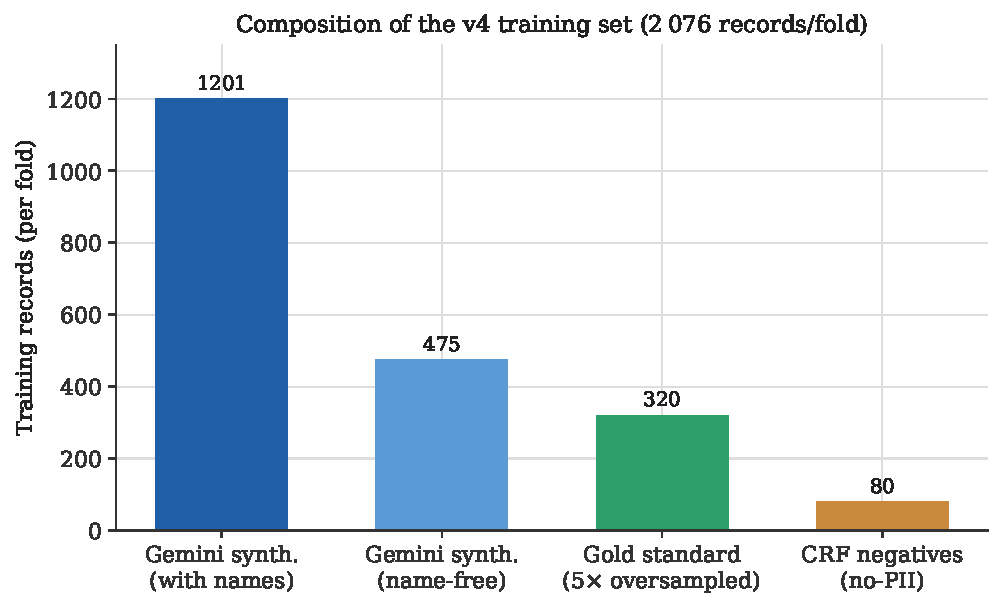
\includegraphics[width=0.82\textwidth]{figures/fig_data_composition.pdf}
\caption{Composition of the final (v4) training set used for the headline result. The gold standard is oversampled $5\times$ within each fold so that a genuinely small amount of real data is not drowned out by the much larger synthetic pool.}
\label{fig:data-composition}
\end{figure}

The CRF negative samples deserve a brief note, since their purpose is easy to misread. These are cases where the input and output are identical -- text with no PII to redact -- included specifically so the model does not learn the degenerate shortcut of redacting \emph{something} in every note regardless of whether anything is actually present. Early experimentation without any negative samples produced a mild but consistent over-tagging tendency on notes with genuinely sparse PII content; adding a modest number of negatives (80, matching roughly the scale of the gold set) resolved this without requiring a much larger negative pool.

The 5$\times$ oversampling of the gold standard within each training fold is a deliberate, if slightly inelegant, design choice rather than a principled one. Without it, the 64 real notes per fold are outnumbered by synthetic data more than 25 to 1, and while the synthetic data is stylistically close to the gold distribution, it is not identical to it; oversampling the real data is a cheap way to keep the model anchored to genuine clinical writing without having to tune a more sophisticated loss-reweighting scheme. Whether a more principled reweighting would do meaningfully better is an open question this thesis did not have the annotated data to answer rigorously, since any such tuning would itself need a validation set independent of the final test folds.

Total cost of the synthetic generation across all versions, v2 and v4 combined, was roughly \$15 in Gemini API credits for approximately 1800 valid generated cases -- a cost low enough that, in a production setting, generating an order of magnitude more style-anchored data would still be inexpensive relative to the cost of additional manual annotation.

% ======================================================================
\chapter{Methodology}
\label{ch:method}
% ======================================================================

This chapter describes how the models were actually trained and evaluated: the task formulation, the two-phase training pipeline, model and hyperparameter configuration, the chat-template mechanics that turned out to matter more than expected, and the cross-validation protocol used to obtain the headline results.

\section{Task Formulation}

As introduced in Chapter~\ref{ch:intro}, the task is framed as inline redaction rather than span extraction: the model receives the full text of a clinical note as a user turn and is expected to produce, as its assistant turn, the same note with every PII span replaced by its category placeholder. This formulation was chosen specifically to match the reference paper's task definition and evaluation metric exactly, so that a macro-F1 number computed on this thesis's model output is directly comparable to a macro-F1 number computed on the reference paper's zero-shot output, without any translation layer between the two evaluation setups.

\section{Two-Phase Training Pipeline}

Training proceeds in two phases, following a pattern common in domain-adaptive fine-tuning: a first phase that adapts the base model's general language modeling to the target domain's vocabulary and register, and a second phase that teaches the specific downstream task on top of that adapted base.

\textbf{Phase 1 -- Continual Pre-Training (CPT).} Before any redaction-specific training, the base Llama-3.2-3B model is further pretrained, self-supervised, on Italian clinical text drawn from \texttt{NLP-FBK/dyspnea-clinical-notes} and \texttt{praiselab-picuslab/DART}, producing a LoRA adapter (\texttt{llama-3.2-3b-dart-sft}) that is then merged into the base weights to form a single Italian-clinical-adapted checkpoint. This phase was inherited from earlier project work rather than re-run for this thesis, and its outputs (the merged checkpoint stored locally as \texttt{temp\_merged\_phase1/}) serve as the starting point for Phase 2. The intent of this phase is purely distributional: give the model more exposure to Italian medical vocabulary, abbreviation conventions, and sentence structure before it is asked to perform the redaction task specifically, rather than expecting the redaction fine-tuning step to teach both domain vocabulary and the task simultaneously from a much smaller dataset.

\textbf{Phase 2 -- Redaction Supervised Fine-Tuning (SFT).} Starting from the merged Phase 1 checkpoint, a second LoRA adapter is trained specifically on the redaction task, using the training data composition described in Chapter~\ref{ch:data}. This is the phase all of the headline results in this thesis refer to, and the one described in detail in the remainder of this chapter.

\section{Model Configuration}
\label{sec:model-config}

Both models fine-tuned in this thesis -- \texttt{meta-llama/Llama-3.2-3B} (with the Phase 1 CPT adapter merged in) and, for the cross-architecture comparison, \texttt{google/gemma-3-1b-it} -- use an identical LoRA and quantization configuration, summarized in Table~\ref{tab:model-config}.

\begin{table}[htbp]
\centering
\caption{LoRA and quantization configuration (identical for both base models).}
\label{tab:model-config}
\begin{tabular}{p{5.2cm}p{7.8cm}}
\toprule
Setting & Value \\
\midrule
LoRA rank $r$ & 16 \\
LoRA alpha & 32 \\
LoRA dropout & 0.05 \\
Target modules & \texttt{q\_proj}, \texttt{k\_proj}, \texttt{v\_proj}, \texttt{o\_proj}, \texttt{gate\_proj}, \texttt{up\_proj}, \texttt{down\_proj} \\
Quantization & 4-bit NF4, double quantization \\
Compute dtype & bfloat16 \\
Trainable parameters (Llama-3.2-3B) & $\approx$52M ($\approx$1.7\% of base) \\
\bottomrule
\end{tabular}
\end{table}

Targeting all seven of the attention and MLP projection matrices, rather than only the attention projections as is sometimes done to save memory, was a deliberate choice: early experimentation with attention-only LoRA (used out of necessity for the Gemma-3~4B attempt discussed in Section~\ref{sec:gemma4b-oom}) produced noticeably less capable adaptation on this task, consistent with the intuition that a redaction task benefits from adapting the MLP layers' capacity to represent domain-specific lexical patterns, not just the attention layers' capacity to route information between tokens.

\section{Chat Template and Assistant-Only Loss}
\label{sec:chat-template}

Getting the chat template right turned out to be one of the more finicky parts of this project, and is worth documenting in some detail because the failure mode when it is wrong is silent rather than a crash. The training data uses a Llama-3-style template with explicit generation markers:

\begin{lstlisting}[language={},basicstyle=\ttfamily\scriptsize]
<|begin_of_text|><|start_header_id|>system<|end_header_id|>
{system}<|eot_id|>
<|start_header_id|>user<|end_header_id|>
{note}<|eot_id|>
<|start_header_id|>assistant<|end_header_id|>
{% generation %}{redacted}<|eot_id|>{% endgeneration %}
\end{lstlisting}

The \texttt{\{\% generation \%\}...\{\% endgeneration \%\}} block, combined with TRL's \texttt{assistant\_only\_loss=True} setting, restricts the training loss to the tokens inside that block -- that is, only the redacted output -- rather than computing loss over the entire sequence including the input note and the chat-template scaffolding tokens. Without this restriction, the model is penalized for its inability to predict the input note it is given (which is, definitionally, not something it should be learning to predict at all, since it is provided as context), and in early experimentation this diluted the effective training signal on the part of the sequence that actually matters, the redacted output. Getting the generation markers to align exactly with the assistant turn boundaries, and not, for instance, accidentally including the closing \texttt{<|eot\_id|>} token inside the loss-masked region or leaving it outside, required some trial and error against the specific tokenizer version in use; a mismatch here does not raise an error, it just quietly trains a slightly worse model, which is a frustrating thing to debug after the fact.

\section{Training Hyperparameters}

Table~\ref{tab:hyperparams} lists the hyperparameters used for Phase 2 training, held constant across the v3 and v4 data configurations and across both base model architectures, so that any performance difference between configurations can be attributed to the data rather than to a confounded hyperparameter change.

\begin{table}[htbp]
\centering
\caption{Phase 2 (redaction SFT) training hyperparameters.}
\label{tab:hyperparams}
\begin{tabular}{ll}
\toprule
Setting & Value \\
\midrule
Epochs & 2 \\
Per-device batch size & 1 \\
Gradient accumulation steps & 16 (effective batch size 16) \\
Learning rate & $5 \times 10^{-5}$, cosine schedule \\
Warmup steps & 50 \\
Max sequence length & 1536 tokens \\
Loss & Assistant-only (Section~\ref{sec:chat-template}) \\
Precision & bfloat16 mixed precision \\
\bottomrule
\end{tabular}
\end{table}

A single training run, under this configuration, takes approximately 50 minutes on an RTX~4070~Ti (12\,GB). The choice of 2 epochs rather than more was informed by early smoke testing: with roughly 2000 training records per fold and a task that is closer to format-adaptation than to learning entirely new knowledge, additional epochs beyond 2 showed diminishing and, in a couple of trial runs, slightly negative returns on held-out performance, consistent with the model beginning to overfit the specific phrasing of the synthetic data rather than the underlying redaction behavior.

\section{Inference Configuration}

At inference time, generation uses greedy decoding (\texttt{do\_sample=False}) for determinism, with \texttt{repetition\_penalty} left at 1.0. This last setting is not the default choice one might reach for -- a repetition penalty above 1.0 is common practice to discourage degenerate looping -- but early experimentation found that values above 1.0 actively suppressed the end-of-sequence token often enough to cause runaway generation past the intended output length, presumably because the redacted output legitimately does contain some repeated tokens (e.g.\ multiple instances of the same placeholder tag in a densely-redacted note) that a repetition penalty discourages regardless of whether the repetition is appropriate. Both of Llama-3's end-of-sequence token variants (\texttt{<|end\_of\_text|>} and \texttt{<|eot\_id|>}) are registered as valid stopping tokens, since relying on only one of the two occasionally let generation run on unnecessarily. Maximum new tokens is set to 1024, sufficient headroom for redacted outputs that are typically close in length to their roughly 1500--3500 character inputs.

\section{Evaluation Protocol}

Per-note, per-category precision, recall, and F1 are computed exactly as described in Section~\ref{sec:eval-metric}, using the deterministic placeholder-counting metric from the reference paper. Two evaluation regimes are used across the experiments reported in Chapter~\ref{ch:results}.

\textbf{Single held-out split.} An early evaluation regime, used for the v2 and v3 iterations during development, holds out 16 of the 80 notes (seed 42) as a fixed test set and trains on the remaining 64. This is fast to run and was useful for rapid iteration on the data pipeline, but Section~\ref{sec:v3-cv} shows exactly how misleading a single 16-note split can be relative to the same model's behavior under cross-validation.

\textbf{5-fold cross-validation.} The headline results in this thesis use \texttt{scikit-learn}'s \texttt{KFold} with \texttt{n\_splits=5}, \texttt{shuffle=True}, \texttt{random\_state=42}, giving five folds of 16 test notes each, with the remaining 64 notes (plus the full synthetic and negative-sample pools) used for training in each fold. Across the five folds, every one of the 80 gold notes is evaluated exactly once as part of a held-out test set, so the aggregated result reflects performance across the entire gold standard rather than one arbitrarily chosen subset of it. Aggregated per-category and macro statistics are reported as mean $\pm$ standard deviation across the five folds. A full 5-fold CV run, retraining the model from the Phase 1 checkpoint five separate times, takes approximately six hours on the same RTX~4070~Ti.

The decision to move from single-split to 5-fold evaluation partway through this project was not originally planned; it followed directly from a single-split result (macro-F1 0.692, reported in Section~\ref{sec:v3-single-split}) that looked, on its face, like a clear and comfortable win over the reference paper's best baseline, and that did not survive being re-evaluated across five different held-out subsets of the same 80 notes. That episode is discussed at more length in Section~\ref{sec:iteration-timeline}, both because it materially changed how the rest of the project was run and because it is, I think, a useful cautionary example for anyone evaluating a model against an 80-note benchmark.

% ======================================================================
\chapter{Experiments and Results}
\label{ch:results}
% ======================================================================

This chapter reports the experimental results, starting with the development timeline that led to the final configuration -- included deliberately, not just as a narrative device, since two of the failures along the way (the no-gold control and the single-split-vs-CV discrepancy) are themselves informative results -- followed by the headline 5-fold cross-validation numbers, the head-to-head comparison with the reference paper, the cross-architecture comparison, and a documented negative result on model scaling.

\section{Development Timeline}
\label{sec:iteration-timeline}

Figure~\ref{fig:iteration-timeline} traces macro-F1 across the successive iterations of this project, from the very first (unsuccessful) task formulation through the final 5-fold cross-validated result. It is worth walking through this progression explicitly, because several of the intermediate points reflect design decisions that are not obvious in hindsight and that materially shaped the final methodology described in Chapter~\ref{ch:method}.

\begin{figure}[htbp]
\centering
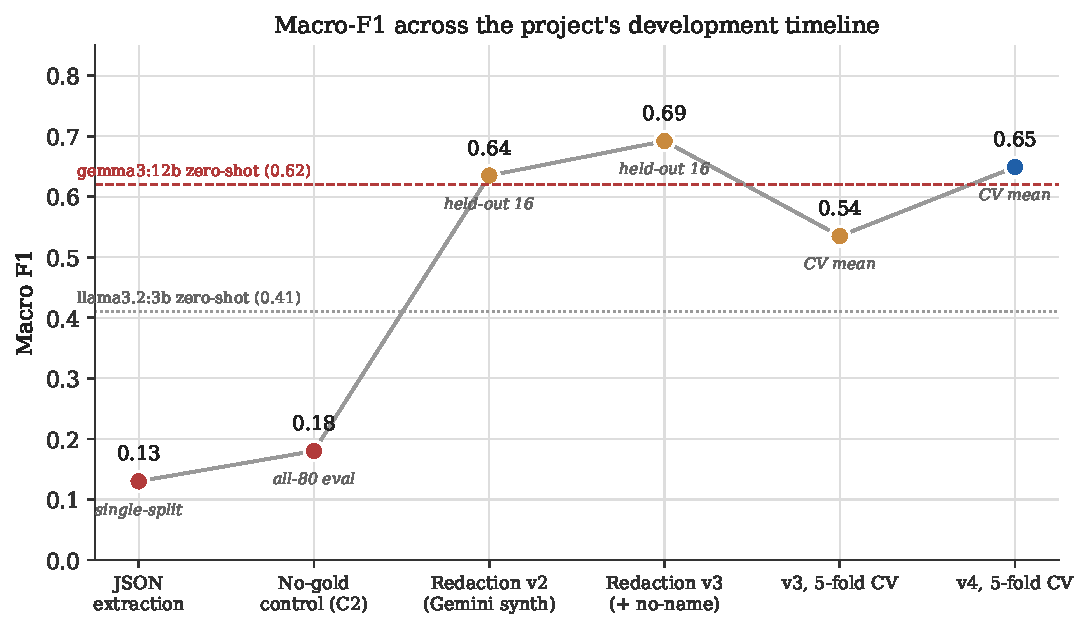
\includegraphics[width=0.92\textwidth]{figures/fig_iteration_timeline.pdf}
\caption{Macro-F1 across the project's development timeline. Note that the two rightmost points (5-fold CV) are evaluated under a stricter, more representative protocol than the three ``held-out 16'' points to their left, which is why the apparent regression from 0.69 to 0.54 is partly an artifact of evaluation methodology rather than a genuine drop in model quality (see Section~\ref{sec:v3-cv}).}
\label{fig:iteration-timeline}
\end{figure}

The first attempt at Phase 2 framed the task as structured extraction: the model was asked to output a JSON list of entities with type labels and short context snippets, rather than a redacted version of the full note. This failed for reasons that, in retrospect, are fairly generic problems with getting a fine-tuned generative model to emit valid structured output reliably: a greedy regular expression used during parsing sometimes captured trailing garbage past the intended JSON object, matching a generated context snippet back to its exact location in the source note was ambiguous whenever a phrase appeared more than once, and the model did not reliably learn to emit an end-of-sequence token at the right point, leading to runaway generation. Macro-F1 on cross-validation for this formulation was approximately 0.13, and after a certain amount of effort trying to patch the parsing and generation-length issues individually, the more fundamental decision to switch to the redaction-as-generation formulation (matching the reference paper) resolved most of these problems at once, simply by removing the need for exact span-location matching.

The redaction formulation was then trained on an early, unconditioned synthetic dataset (\texttt{synthetic\_clinical\_1000.json}, distinct from the style-anchored \texttt{synthetic\_v2} data described in Chapter~\ref{ch:data}) together with the gold notes and CRF negatives. A first sanity-check evaluation, unfortunately conducted against the training set itself rather than a genuine held-out set, showed macro-F1 0.60 -- a number that, correctly, should never have been reported as a benchmark result, and is included here only as a data point in the iteration history rather than as evidence of anything.

\subsection{The No-Gold Control Experiment}
\label{sec:no-gold-control}

The critical diagnostic experiment of this project, referred to throughout as C2, trained the redaction model on the unconditioned synthetic data plus CRF negatives \emph{with no gold notes included at all}, then evaluated it on the full 80-note gold set. The result was unambiguous: macro-F1 0.18, below every zero-shot baseline reported in the reference paper, including their weakest model. Inspecting the model's raw outputs on a sample of gold notes showed two failure patterns: on some notes the model copied the input essentially unchanged, emitting no redaction at all, and on others it generated catastrophic repeating loops of the \NOME{} placeholder tag with no relationship to the actual content. The most plausible explanation, based on comparing the surface style of the synthetic training data against the gold notes, is that the model had learned a spurious correlation between \emph{surface style} and \emph{whether redaction was expected}, rather than learning the underlying redaction task itself -- effectively, ``text that looks like the synthetic training distribution gets redacted; text that looks like something else, including real clinical prose, does not.''

This is, as far as I can tell, the single most consequential finding of the entire project, more consequential in practice than the final headline F1 number, because it directly motivated the style-anchored generation approach described in Section~\ref{sec:style-anchoring} and because it is a failure mode that would be easy to miss without a control experiment specifically designed to isolate it. A model trained on synthetic data alone that happens to score reasonably on a single held-out split of \emph{synthetic} data could look successful right up until it is deployed on the real, differently-styled text it was actually built to handle.

\subsection{From Style-Anchored Data to a First Promising Result}
\label{sec:v3-single-split}

Replacing the unconditioned synthetic batch with the style-anchored \texttt{synthetic\_v2} data (Section~\ref{sec:style-anchoring}) and re-training on the same 64/16 held-out split immediately reversed the collapse: macro-F1 rose to 0.635. Adding the 254 name-free cases described in Section~\ref{sec:nome-overrep} to address the \NOME{} over-representation problem raised it further, to 0.692 on the same held-out 16 notes -- comfortably above the reference paper's best zero-shot result of 0.620, with per-category gains of +0.17 on \ETA{} and +0.21 on \DATA{} against the paper's best model, at the cost of a substantial -0.31 deficit on \NOME{} specifically. Table~\ref{tab:v3-single-split} gives the full per-category breakdown for this result.

\begin{table}[htbp]
\centering
\caption{v3 single-split held-out result (16 notes, seed 42).}
\label{tab:v3-single-split}
\begin{tabular}{lrrrrrr}
\toprule
Category & TP & FP & FN & Precision & Recall & F1 \\
\midrule
\NOME{} & 4 & 4 & 4 & 0.500 & 0.500 & 0.500 \\
\ETA{} & 11 & 10 & 6 & 0.524 & 0.647 & 0.579 \\
\DATA{} & 3 & 0 & 1 & 1.000 & 0.750 & 0.857 \\
\LUOGO{} & 5 & 1 & 1 & 0.833 & 0.833 & 0.833 \\
\midrule
\textbf{Macro} & & & & & & \textbf{0.692} \\
\bottomrule
\end{tabular}
\end{table}

At this point in the project, a macro-F1 of 0.692 on 16 held-out notes looked like a clean, sizable win. It is worth being honest that this was also the point at which it would have been tempting to stop and write it up as the final result. What happened next is the reason this thesis reports 5-fold CV numbers as its headline result instead.

\subsection{v3: 5-Fold Cross-Validation Reveals High Variance}
\label{sec:v3-cv}

Re-evaluating the same v3 training configuration under 5-fold cross-validation -- training five separate models, each on a different 64-note subset, and evaluating each on its corresponding 16-note held-out fold -- told a considerably less comfortable story. Table~\ref{tab:v3-cv-folds} shows the per-fold macro-F1.

\begin{table}[htbp]
\centering
\caption{v3, per-fold macro-F1 under 5-fold cross-validation.}
\label{tab:v3-cv-folds}
\begin{tabular}{lrrrrr}
\toprule
Fold & 1 & 2 & 3 & 4 & 5 \\
\midrule
Macro-F1 & 0.595 & 0.643 & 0.460 & 0.690 & 0.291 \\
\bottomrule
\end{tabular}
\end{table}

The aggregated result is macro-F1 $0.535 \pm 0.144$ -- below the reference paper's 0.620, and with a standard deviation across folds large enough that the single-split result of 0.692 from Section~\ref{sec:v3-single-split} is revealed to have simply landed on a favorable split, specifically Fold 4's 16 notes, rather than reflecting the model's typical behavior. Fold 5 in particular collapsed to 0.291, driven by a complete failure on \DATA{} (F1 = 0.000, the model identified no dates correctly in that fold's test notes) and a flood of false-positive \LUOGO{} placeholders. Excluding Fold 5 as an outlier would raise the mean to roughly 0.597, still short of the paper's best result, and in any case selectively excluding an inconvenient fold after the fact is not a defensible way to report a result.

Two things stand out from this table. First, the fold-to-fold range -- from 0.291 to 0.690, a spread of 40 percentage points on the same training recipe -- is a direct consequence of the small size of the underlying test set; with only 16 notes per fold, a handful of unusually hard or unusually easy notes can move the macro-F1 substantially. Second, and more constructively, \DATA{}'s per-category standard deviation (0.309) was by far the largest of the four categories, ranging from a perfect 0.933 in Fold 4 down to 0.000 in Fold 5, suggesting the model's date-handling behavior specifically had not yet generalized reliably across the range of date formats and contexts present in the full 80-note set. This observation directly motivated the v4 data expansion described next.

\section{v4: The Headline Result}
\label{sec:v4-headline}

Having diagnosed v3's high variance as plausibly connected to insufficient synthetic data volume -- specifically, insufficient coverage of the range of surface forms within the already-validated style-anchored approach -- the v4 configuration doubled the synthetic pool, adding \texttt{synthetic\_v4\_named\_more.json} (577 additional with-name cases) and \texttt{synthetic\_v4\_noname\_more.json} (221 additional name-free cases) to the existing v3 pool, for a total of 1201 with-name and 475 name-free synthetic cases (2076 total training records per fold, as detailed in Table~\ref{tab:data-composition-thesis}). All other hyperparameters, and the same KFold seed, were held fixed relative to v3, so that fold-by-fold comparison between the two configurations is meaningful.

\begin{figure}[htbp]
\centering
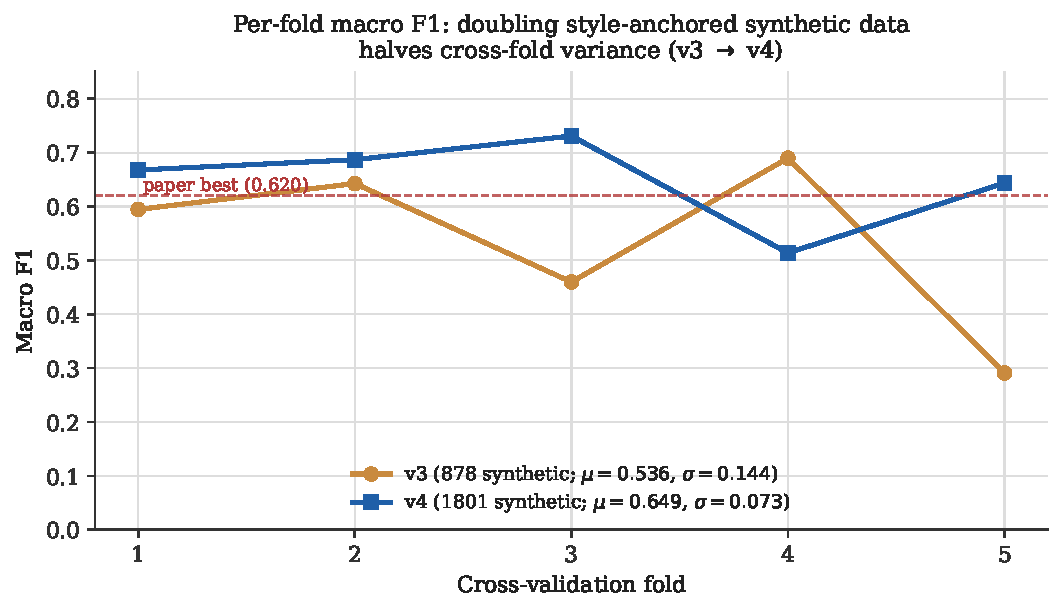
\includegraphics[width=0.92\textwidth]{figures/fig_fold_variance.pdf}
\caption{Per-fold macro-F1, v3 versus v4. Doubling the volume of style-anchored synthetic data raised the mean by 0.114 and, more strikingly, roughly halved the standard deviation across folds, from 0.144 to 0.073.}
\label{fig:fold-variance}
\end{figure}

Table~\ref{tab:v4-fold-comparison} and Figure~\ref{fig:fold-variance} show the fold-by-fold comparison. The mean rose from 0.535 to 0.649 (+0.114), and the standard deviation across folds fell from 0.144 to 0.073 -- very close to a halving. Individually, three folds improved substantially (Fold 3: +0.271; Fold 5: +0.353, recovering from the v3 collapse), one improved modestly (Fold 1: +0.073; Fold 2: +0.044), and one fold that had been the strongest under v3 became the weakest under v4 (Fold 4: $-0.176$, driven by a specific collapse on \DATA{} in that fold, F1 = 0.20). This last point matters: variance reduction under v4 is real and substantial in aggregate, but it did not eliminate fold-localized failure, it relocated where the weakest fold occurred.

\begin{table}[htbp]
\centering
\caption{Per-fold macro-F1, v3 vs.\ v4.}
\label{tab:v4-fold-comparison}
\begin{tabular}{lrrr}
\toprule
Fold & v3 & v4 & $\Delta$ \\
\midrule
1 & 0.595 & 0.668 & +0.073 \\
2 & 0.643 & 0.687 & +0.044 \\
3 & 0.460 & 0.731 & +0.271 \\
4 & 0.690 & 0.514 & $-0.176$ \\
5 & 0.291 & 0.644 & +0.353 \\
\midrule
\textbf{Mean} & \textbf{0.535} & \textbf{0.649} & \textbf{+0.114} \\
\textbf{Std.\ dev.} & \textbf{0.144} & \textbf{0.073} & \textbf{$-0.071$} \\
\bottomrule
\end{tabular}
\end{table}

Table~\ref{tab:v4-aggregate} gives the full aggregated per-category precision, recall, and F1 for v4, the configuration used for all headline comparisons in the remainder of this chapter.

\begin{table}[htbp]
\centering
\caption{v4 aggregated per-category results (mean $\pm$ std.\ across 5 folds).}
\label{tab:v4-aggregate}
\begin{tabular}{lccc}
\toprule
Category & Precision & Recall & F1 \\
\midrule
\NOME{} & $0.640 \pm 0.216$ & $0.856 \pm 0.198$ & $0.714 \pm 0.186$ \\
\ETA{} & $0.615 \pm 0.109$ & $0.512 \pm 0.158$ & $0.554 \pm 0.129$ \\
\DATA{} & $0.680 \pm 0.264$ & $0.533 \pm 0.278$ & $0.536 \pm 0.191$ \\
\LUOGO{} & $0.914 \pm 0.171$ & $0.700 \pm 0.130$ & $0.790 \pm 0.140$ \\
\midrule
\textbf{Macro F1} & & & \textbf{0.649 $\pm$ 0.073} \\
\bottomrule
\end{tabular}
\end{table}

\section{Head-to-Head Comparison with the Reference Paper}

Figure~\ref{fig:leaderboard} and Table~\ref{tab:head-to-head} place the v4 result directly alongside the five zero-shot baselines from Miranda et al., along with the Gemma-3~1B cross-architecture result discussed in the next section. The v4 model's macro-F1 of 0.649 exceeds the reference paper's best result, \texttt{gemma3:12b} at 0.620, by 0.029 absolute, using a model roughly four times smaller and, unlike the zero-shot baselines, requiring an upfront training cost of a few hours on consumer hardware in exchange for that improvement.

\begin{figure}[htbp]
\centering
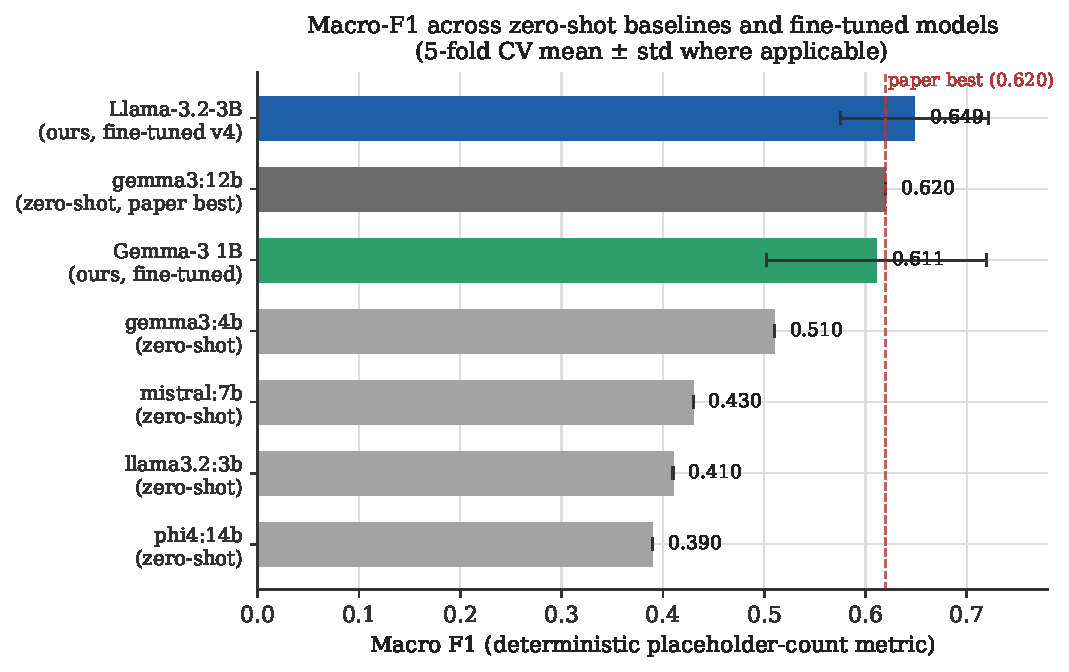
\includegraphics[width=0.92\textwidth]{figures/fig_leaderboard.pdf}
\caption{Macro-F1 across all zero-shot baselines from the reference paper and both fine-tuned models from this thesis. Error bars on the fine-tuned models show $\pm 1$ standard deviation across the 5 cross-validation folds; the zero-shot baselines are single-run results with no reported variance.}
\label{fig:leaderboard}
\end{figure}

\begin{table}[htbp]
\centering
\caption{Head-to-head comparison: reference-paper zero-shot baselines vs.\ this thesis's fine-tuned models.}
\label{tab:head-to-head}
\small
\begin{tabular}{p{3.3cm}p{1.3cm}p{1.8cm}rrrr}
\toprule
Model & Params & Approach & \NOME{} & \ETA{} & \DATA{} & \LUOGO{} \\
\midrule
phi4:14b & 14B & zero-shot & 0.44 & 0.23 & 0.33 & 0.55 \\
llama3.2:3b & 3B & zero-shot & 0.53 & 0.41 & 0.29 & 0.41 \\
mistral:7b & 7B & zero-shot & 0.77 & 0.24 & 0.37 & 0.34 \\
gemma3:4b & 4B & zero-shot & 0.73 & 0.30 & 0.27 & 0.75 \\
\textbf{gemma3:12b} (paper best) & \textbf{12B} & zero-shot & \textbf{0.81} & 0.14 & 0.65 & \textbf{0.88} \\
\midrule
Gemma-3 1B (ours) & 1B & fine-tuned & 0.59 & \textbf{0.75} & 0.58 & 0.52 \\
\textbf{Llama-3.2-3B v4} (ours) & \textbf{3B} & fine-tuned & 0.71 & 0.55 & 0.54 & 0.79 \\
\bottomrule
\end{tabular}
\normalsize

\vspace{0.3cm}
\small
Macro-F1: phi4:14b 0.39, llama3.2:3b 0.41, mistral:7b 0.43, gemma3:4b 0.51, gemma3:12b \textbf{0.620}, Gemma-3 1B (ours) $0.611 \pm 0.109$, Llama-3.2-3B v4 (ours) \textbf{$0.649 \pm 0.073$}.
\end{table}

The per-category picture is more nuanced than the macro number alone suggests, and Figure~\ref{fig:per-category} makes the trade-off visible directly. Relative to \texttt{gemma3:12b}, the v4 model gains +0.144 on \ETA{} (0.554 vs.\ 0.14 --- the category the reference paper itself flags as universally weak across zero-shot models) and closes most, though not all, of the gap on \NOME{} (from a $-0.31$ deficit at the v3 stage to $-0.10$ at v4) and \LUOGO{} (from $-0.31$ to $-0.09$). \DATA{} sits roughly 0.11 behind the paper's best result. No single category shows the fine-tuned model uniformly dominating; the aggregate improvement comes from a large, decisive win on the category the zero-shot approach handles worst, combined with narrowing, without fully closing, the gap on the categories zero-shot handles best.

\begin{figure}[htbp]
\centering
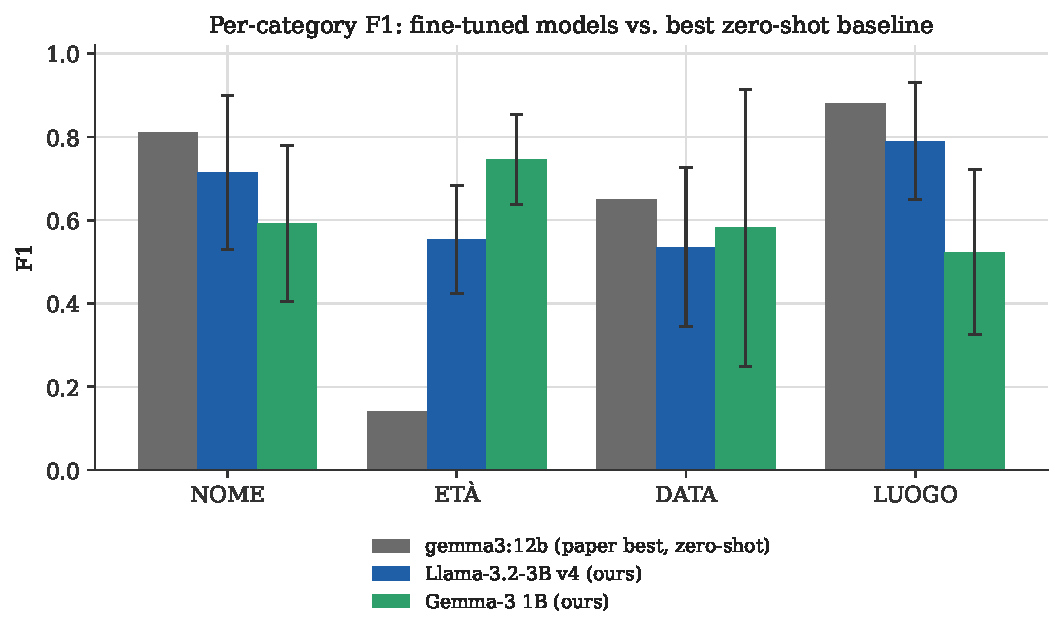
\includegraphics[width=0.92\textwidth]{figures/fig_per_category.pdf}
\caption{Per-category F1: the reference paper's best zero-shot model against both fine-tuned models from this thesis. The largest single gain, on \ETA{}, corresponds to the category the reference paper explicitly identifies as the weakest point of zero-shot prompting.}
\label{fig:per-category}
\end{figure}

Figure~\ref{fig:precision-recall} shows the precision--recall operating point of the v4 model for each category individually. \LUOGO{} sits in a distinctive high-precision, moderate-recall regime (precision 0.914): when the model does emit a \LUOGO{} tag, it is very likely correct, but it under-tags roughly 30\% of actual locations. \NOME{}, by contrast, sits at high recall but moderate precision, reflecting a mild over-tagging tendency that the name-free data (Section~\ref{sec:nome-overrep}) reduced substantially from earlier iterations but did not eliminate entirely.

\begin{figure}[htbp]
\centering
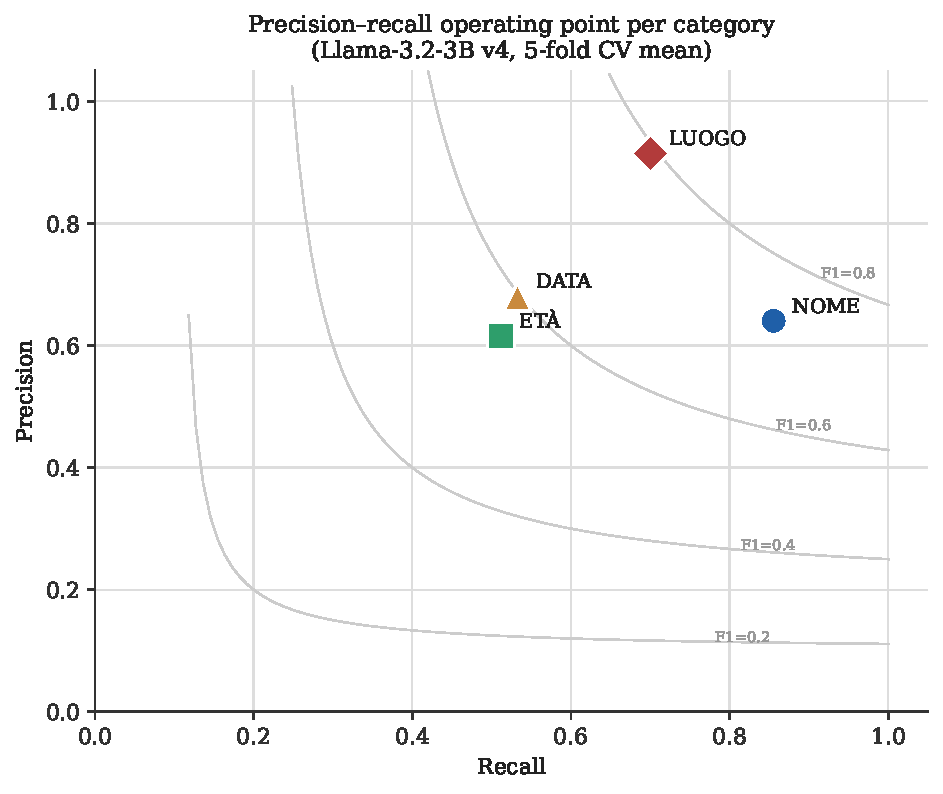
\includegraphics[width=0.68\textwidth]{figures/fig_precision_recall.pdf}
\caption{Precision--recall operating point per category for the v4 model (5-fold CV mean). Grey curves are iso-F1 contours.}
\label{fig:precision-recall}
\end{figure}

\section{Cross-Architecture Comparison: Gemma-3 1B}

To separate the effect of the training \emph{method} from the effect of base-model scale, the identical v4 pipeline -- same data, same hyperparameters, same 5-fold split -- was applied to \texttt{google/gemma-3-1b-it}, an instruction-tuned 1-billion-parameter model roughly three times smaller than the Llama-3.2-3B base. Table~\ref{tab:gemma1b-aggregate} and Figure~\ref{fig:architecture-comparison} show the result.

\begin{table}[htbp]
\centering
\caption{Gemma-3 1B, aggregated per-category results (mean $\pm$ std.\ across 5 folds).}
\label{tab:gemma1b-aggregate}
\begin{tabular}{lc}
\toprule
Category & F1 \\
\midrule
\NOME{} & $0.592 \pm 0.187$ \\
\ETA{} & $\mathbf{0.745 \pm 0.108}$ \\
\DATA{} & $0.582 \pm 0.332$ \\
\LUOGO{} & $0.523 \pm 0.199$ \\
\midrule
\textbf{Macro F1} & \textbf{0.611 $\pm$ 0.109} \\
\bottomrule
\end{tabular}
\end{table}

\begin{figure}[htbp]
\centering
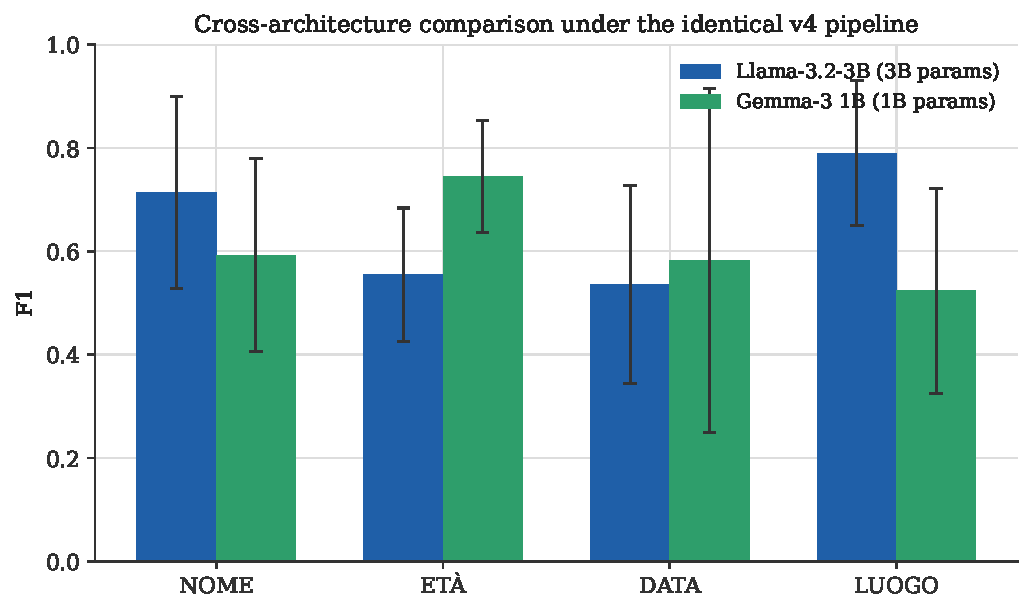
\includegraphics[width=0.85\textwidth]{figures/fig_architecture_comparison.pdf}
\caption{Cross-architecture comparison under the identical v4 pipeline: Llama-3.2-3B versus Gemma-3 1B.}
\label{fig:architecture-comparison}
\end{figure}

At 0.611, the 1B Gemma model lands within one standard deviation of the reference paper's 12B zero-shot result (0.620) and within its own standard deviation of the 3B Llama result (0.649), despite having twelve times fewer parameters than the zero-shot baseline it is being compared against and roughly a third as many as the Llama model trained under the identical pipeline. Interestingly, Gemma-3~1B's \ETA{} score, 0.745, is not just its own strongest category but the single highest \ETA{} score of any model in this comparison, including the larger fine-tuned Llama model -- suggestive, though not conclusive on a single 1B-vs-3B comparison, that Gemma-3's instruction-tuning baseline may already have somewhat better-calibrated handling of numeric age expressions before any task-specific fine-tuning is applied, an advantage that fine-tuning then amplifies rather than originates.

Two aspects of the Gemma-3~1B result temper how much weight this comparison can bear. First, its cross-fold variance (std.\ 0.109) is noticeably higher than the Llama-3.2-3B v4 result (std.\ 0.073), consistent with a smaller model being more sensitive to which particular 16 notes happen to land in a given test fold -- the same Fold~5 that recovered strongly for Llama v4 saw Gemma-3~1B collapse on \DATA{} specifically (F1 = 0.000, three false-positive tags against four missed real dates). Second, \LUOGO{} is markedly weaker than the Llama result (0.523 vs.\ 0.790), plausibly reflecting less capacity, at 1B parameters, to memorize the range of Italian place names, hospital names, and address formats the task requires.

\section{A Documented Negative Result: Gemma-3 4B}
\label{sec:gemma4b-oom}

An attempt was made to extend the cross-architecture comparison one step further, to \texttt{google/gemma-3-4b}, a natural intermediate point between the 1B and Llama's 3B. This attempt did not succeed, and is reported here because the reason it failed is itself informative about deploying small language models under real hardware constraints rather than in a research-cluster setting.

Even with attention-only LoRA (dropping the MLP target modules used elsewhere in this thesis), a reduced maximum sequence length of 768 tokens, gradient checkpointing enabled, a paged 8-bit AdamW optimizer, and \texttt{assistant\_only\_loss} disabled, training ran out of GPU memory specifically at the cross-entropy loss computation step. The root cause is Gemma-3's unusually large vocabulary -- 262,144 tokens, roughly ten times larger than Llama-3's -- which forces the logits tensor for a training batch to have shape \texttt{[sequence\_length, 262144]}. In 32-bit precision (required for numerically stable cross-entropy), this tensor alone consumes close to 800\,MB per batch element, with a comparable amount again required for its gradient during backpropagation, on top of the roughly 9.5\,GB already consumed by the quantized weights and activations before the loss step is even reached. On a 12\,GB card, there is simply no room left.

This is, in a narrow sense, a negative result -- Gemma-3~4B does not fit in the hardware budget this thesis targets -- but I think it is worth reporting as a positive finding about model selection under real deployment constraints: Llama-3.2-3B, at roughly 3.2B parameters and a comparatively modest 128K-token vocabulary, fits comfortably within a 12\,GB budget, while Gemma-3~4B, despite having only somewhat more parameters, does not, because vocabulary size interacts with training memory in a way that raw parameter count alone does not capture. For a practitioner choosing a base model under a fixed, single-consumer-GPU hardware budget, this is arguably as decision-relevant as the F1 comparisons elsewhere in this chapter. Fitting Gemma-3~4B on 12\,GB would likely require chunked cross-entropy computation (for instance via a fused kernel such as Liger) or layer offloading, neither of which was implemented for this thesis.

\section{Training Cost and Reproducibility}

Table~\ref{tab:cost-summary} summarizes the compute and API cost of the full experimental pipeline. All random seeds are fixed at 42 throughout (data splitting, synthetic-data sampling where applicable, and model initialization where the underlying libraries expose a seed), and the exact train/test indices used for the single-split evaluations in Section~\ref{sec:v3-single-split} are persisted to \texttt{data/test\_indices\_seed42.json} for reproducibility.

\begin{table}[htbp]
\centering
\caption{Compute and API cost summary.}
\label{tab:cost-summary}
\begin{tabular}{ll}
\toprule
Item & Cost \\
\midrule
GPU & 1$\times$ RTX 4070 Ti (12\,GB) \\
Single training run & $\approx$50 minutes \\
Single 80-note evaluation pass & $\approx$60 minutes \\
Full 5-fold CV (train + eval, one configuration) & $\approx$6 hours \\
Gemini API cost (all synthetic data, v2 + v4) & $\approx$\$15, $\approx$1800 valid cases \\
Adapter + merged-model storage & $\approx$200\,MB per configuration \\
\bottomrule
\end{tabular}
\end{table}

% ======================================================================
\chapter{Discussion}
\label{ch:discussion}
% ======================================================================

\section{Why Fine-Tuning a Small Model Beats a Larger Zero-Shot One}

The result reported in Chapter~\ref{ch:results} -- a 3B fine-tuned model outperforming a 12B zero-shot model on macro-F1 -- is easiest to understand by looking at where the gain actually comes from, rather than treating it as a single undifferentiated number. Almost the entire margin is explained by one category, \ETA{}, where the zero-shot approach struggles specifically because age mentions in Italian clinical prose are lexically ambiguous with other numeric temporal expressions -- \emph{``vent'anni di ipertensione''} (twenty years of hypertension) uses the same surface pattern as an age reference but refers to a duration, not a patient's age, and a model with no task-specific examples of this distinction has to resolve it from general world knowledge alone, which the reference paper's results suggest it does poorly (their best zero-shot \ETA{} score is 0.41; \texttt{gemma3:12b} specifically scores only 0.14). Fine-tuning, even on a training set built mostly from synthetic data, exposes the model to thousands of correctly-labeled instances of exactly this ambiguity, and it resolves a large fraction of it: the v4 model's \ETA{} F1 of 0.554 is a 0.144-point absolute gain over the paper's best zero-shot result, and Gemma-3~1B's \ETA{} score of 0.745 is higher still, at a fraction of the parameter count.

A similar, if less dramatic, story applies to \DATA{}: zero-shot models in the reference paper appear to systematically miss partial or informally expressed dates (\emph{``2017''} on its own, \emph{``l'estate scorsa''}, last summer) that don't match a canonical date-format prior, whereas a model trained on data that deliberately mixes date formats learns to recognize the wider range of surface forms actually used in Italian clinical writing. The general pattern across both categories is that fine-tuning is doing something closer to \emph{disambiguation} than to teaching an entirely new capability from scratch -- the underlying concepts of ``age'' and ``date'' are already well within a 3B or even 1B model's general knowledge; what is missing zero-shot is calibration to how those concepts are specifically expressed, and disambiguated from look-alikes, in this particular register of Italian text.

\section{Why \NOME{} Remains the Hardest Category}

The picture is less favorable for \NOME{}, and it is worth being direct about why, rather than treating the remaining gap as a simple matter of ``needs more training.'' The gold standard contains only 46 \NOME{} entities across all 80 notes, the smallest of the four categories by a wide margin, and those 46 instances have to cover a genuinely hard sub-problem: distinguishing patient names from clinician names, from family-member names mentioned incidentally, and from capitalized non-name terms that happen to appear at the start of a sentence -- all cases that a general-purpose model with broad pretraining on named-entity recognition, like \texttt{gemma3:12b}, likely handles well simply from scale and prior exposure to name-recognition patterns in its much larger pretraining corpus.

The synthetic data used in this thesis, despite the style-anchoring and name-free rebalancing described in Chapter~\ref{ch:data}, still carries structural artifacts that the gold notes do not share as strongly: synthetic with-name cases tend to introduce the patient's name early and repeat it several times via anaphora, whereas gold notes sometimes introduce a name later in the note, or mention it only once. A model trained predominantly on the former pattern may be picking up positional and repetition cues that do not transfer perfectly to the latter. Closing this gap further plausibly requires one of a few things this thesis did not have the resources to pursue: substantially more real annotated data (the most direct fix, but also the most expensive, since it requires expert clinical annotation rather than API calls); explicit augmentation of the existing gold notes that re-positions or varies the repetition pattern of names within otherwise-unchanged text; or constrained generation at inference time using an external name dictionary to catch names the model's own recognition misses. None of these were implemented here, and Section~\ref{sec:future-work} discusses them as concrete next steps rather than speculative ones.

\section{Style Versus Volume: The Central Empirical Finding}

If this thesis has one finding I would want a future practitioner working on a similarly low-resource clinical NLP task to take away, it is the contrast between Section~\ref{sec:no-gold-control}'s no-gold control experiment and Section~\ref{sec:v4-headline}'s v4 result. The former shows that 1000 synthetic notes, generated without any conditioning on the target distribution's actual style, can make a model \emph{worse than doing nothing} -- worse than every zero-shot baseline the reference paper reports, including models the fine-tuned model in question was itself derived from. The latter shows that roughly 1800 synthetic notes, generated with real gold notes embedded as few-shot style anchors and validated against a fairly strict structural gate, not only avoid that collapse but push performance decisively past the strongest zero-shot baseline available.

Both training runs used broadly comparable volumes of synthetic data (1000 unconditioned vs.\ roughly 1700--1800 style-anchored, generated across the v2 and v4 batches). What differed was not scale but distributional match to the target domain. This suggests, at least for this task and this scale of base model, that the marginal value of an additional synthetic training example is close to zero, or actively negative, if that example's surface style diverges meaningfully from the real distribution it is meant to approximate -- and that practitioners facing a similar resource constraint would likely get more benefit from investing effort in a smaller, carefully style-matched synthetic dataset than in simply generating more data from a generic prompt. The doubling of synthetic volume from v3 to v4 (Section~\ref{sec:v4-headline}) does show that, once the style-matching problem is solved, additional volume still has real marginal value -- primarily in the form of reduced cross-fold variance rather than a dramatically higher mean -- but that effect operates on top of the style-matching prerequisite, not as a substitute for it.

\section{This Work Relative to the Reference Paper}

Table~\ref{tab:contribution-summary} summarizes, side by side, what this thesis adds relative to Miranda et al.\ specifically. The comparison is deliberately narrow and structural rather than a general claim about which approach is ``better'' in the abstract: the two approaches trade off differently against a hospital deployment scenario. Zero-shot prompting requires no training data or training infrastructure at all, which matters if even the modest annotation effort behind an 80-note gold standard is unavailable; fine-tuning requires that gold standard (or, as this thesis shows, a much smaller amount of it supplemented with carefully constructed synthetic data) but delivers a smaller, cheaper-to-run model with better performance on the specific task and specific institution's note style it was trained for.

\begin{table}[htbp]
\centering
\caption{This thesis's contribution relative to the reference paper.}
\label{tab:contribution-summary}
\begin{tabular}{p{5.6cm}p{5.6cm}}
\toprule
Miranda et al.\ (2025) & This thesis \\
\midrule
Zero-shot prompting only, no training data required & LoRA fine-tuning, requires the 80-note gold standard plus synthetic augmentation \\
Best result needs a 12B-parameter model & Best result uses a 3B model; a 1B model reaches within statistical noise of the 12B zero-shot result \\
No synthetic data used & Style-anchored, validated synthetic data pipeline; explicit style-vs-volume ablation \\
\ETA{} is the weakest category across every model tested & \ETA{} is among the strongest categories for both fine-tuned models \\
Single train/test protocol implied by zero-shot evaluation & Both single-split and 5-fold CV reported, with CV shown to meaningfully change the picture \\
\bottomrule
\end{tabular}
\end{table}

% ======================================================================
\chapter{Limitations and Future Work}
\label{ch:limitations}
% ======================================================================

\section{Limitations}

\textbf{The gold dataset is small, and this drives most of the observed variance.} Every number in Chapter~\ref{ch:results} ultimately rests on 80 annotated notes, and the 5-fold CV protocol, while considerably more honest than a single split, cannot manufacture information that was never annotated in the first place. Fold-to-fold macro-F1 swings of up to 40 percentage points (Section~\ref{sec:v3-cv}) are a direct symptom of this: with 16 test notes per fold, a handful of unusually hard notes clustering into one fold can move the aggregate score substantially, and there is no way to distinguish, from this data alone, genuine model weakness on a category from an unlucky clustering of hard examples. Expanding the annotated gold set -- even to a few hundred notes -- would likely do more to firm up the reliability of any reported number than further tuning of the training recipe on the current 80.

\textbf{The evaluation is specific to one language, one corpus style, and four categories.} All results are specific to Italian clinical narratives in the E3C/CLinkaRT register. Whether the same fine-tuning approach, and particularly the style-anchored synthetic data pipeline, transfers to other note types (operative reports, discharge summaries with a different structure, nursing notes) or to other languages was not tested and should not be assumed. The four PII categories evaluated here are also a subset of what a real de-identification system would need to cover -- the reference paper notes that a fuller PHI taxonomy includes as many as 19 categories, and this thesis, like the reference paper, is scoped to the four for which the shared gold standard actually has annotations.

\textbf{No constrained decoding at inference time.} The system relies entirely on the fine-tuned model's learned output format; nothing enforces, structurally, that every input token not corresponding to a placeholder is preserved verbatim, or that a name-like token is never accidentally left unredacted. A production deployment handling real patient data would reasonably want a constrained-generation layer (for instance using a library such as \texttt{outlines} or \texttt{lm-format-enforcer}) to guarantee a valid, complete redaction even on adversarial or unusually formatted inputs, rather than trusting the model's learned behavior alone.

\textbf{The synthetic data still carries stylistic artifacts.} Despite the style-anchoring described in Chapter~\ref{ch:data}, synthetic with-name cases systematically place the patient's name early in the note and repeat it more consistently than gold notes do, and the synthetic date distribution likely over-represents recent years (roughly 2017--2024) relative to whatever the true distribution across a hospital's full note archive would look like. A more sophisticated generation pipeline could explicitly match entity-position and temporal distributions from the gold set rather than relying on prompt instructions and post-hoc inspection to approximate them.

\textbf{No comparison against a fine-tuned sequence-labeling (BERT-style) baseline.}
\label{sec:limitations-bert}
The reference paper explicitly notes the absence of a BERT-NER baseline as a limitation of their own study, and this thesis, despite closing the ``no fine-tuned baseline'' gap the paper identifies, inherits this specific limitation unchanged. The English clinical de-identification literature reviewed in Chapter~\ref{ch:related} is overwhelmingly built on exactly this kind of token-classification architecture, and it would report F1 scores under a different, typically stricter, span-overlap metric rather than the placeholder-counting metric used throughout this thesis -- so a direct comparison would require either re-implementing the placeholder-counting metric for a token-classifier's output or re-evaluating the generative models under a span-overlap metric, neither of which was done here. Adding this baseline, under a metric that supports fair comparison to both approaches, is the most obviously missing piece of the picture and is discussed further below.

\section{Future Work}
\label{sec:future-work}

\textbf{A fine-tuned BERT-NER baseline.} The most direct next experiment is to fine-tune an Italian BERT variant, such as \texttt{dbmdz/bert-base-italian-xxl-cased}, as a token classifier on the same 80 gold notes under an equivalent cross-validation protocol. Comparable Italian clinical NER tasks in the literature routinely report F1 above 0.85 for BERT-style token classification, though usually on considerably larger annotated corpora than this thesis's 80 notes, so it is genuinely unclear ahead of time whether such a model would outperform, match, or underperform the generative approach used here once trained on an equally small amount of real data plus a comparable synthetic augmentation strategy. This is, in my view, the single highest-value follow-up experiment left open by this thesis.

\textbf{An Italian-native base model.} Replacing Llama-3.2-3B with Minerva-3B \citep{orlando2024minerva}, trained from scratch with Italian as a first-class pretraining language rather than one component of a larger multilingual mixture, or with a clinically-oriented base model, is a natural next step and one the reference paper itself recommends. Whether Italian-native pretraining specifically helps with the categories this thesis still struggles on -- \NOME{} in particular -- or mainly helps with fluency and vocabulary efficiency without changing the entity-recognition picture much, is an open empirical question.

\textbf{Constrained generation for production deployment.} Adding a constrained-decoding layer, as noted in the limitations above, would move this from a research prototype toward something that could plausibly be trusted with real, un-reviewed patient text, by providing a structural guarantee that redaction output is well-formed rather than relying entirely on learned behavior.

\textbf{An active-learning loop to grow the gold set.} Given how much of the residual uncertainty in this thesis's results traces back to the 80-note gold set's size, a natural next step is to use the current fine-tuned model to pre-annotate additional unlabeled clinical text, route the model's output to a clinician for correction rather than annotation from scratch, and fold the corrected notes back into the gold set -- a standard active-learning pattern that could plausibly reach a few hundred annotated notes at a fraction of the cost of annotating that many from a blank page.

\textbf{A hybrid extraction-plus-generation system.} A system combining a high-precision span extractor (a BERT-NER model, per the point above) with a generative model responsible for producing natural-sounding redacted or surrogate text -- replacing \texttt{[\NOME{}]} with a plausible substitute name rather than a visible tag, for downstream readability -- could plausibly combine the precision advantages typically associated with token classification with the fluent, format-flexible output a generative model provides.

\textbf{Cross-hospital and cross-register generalization.} All data in this thesis, gold and synthetic alike, derives from or is anchored to a single corpus style (E3C/CLinkaRT case-summary-style narratives). Testing the fine-tuned model against clinical text from a different institution, or a structurally different note type such as a nursing progress note or an operative report, would be a meaningful test of whether the fine-tuning gains reported here reflect genuine task competence or a narrower fit to this specific corpus's conventions.

% ======================================================================
\chapter{Conclusion}
\label{ch:conclusion}
% ======================================================================

This thesis set out to answer a question the reference paper posed but did not itself answer: whether a fine-tuned, considerably smaller model could match or beat zero-shot prompting of a large instruction-tuned model on Italian clinical de-identification. Under 5-fold cross-validation on the same 80-note gold standard used by Miranda et al., a LoRA-fine-tuned Llama-3.2-3B reaches macro-F1 $0.649 \pm 0.073$, exceeding their best zero-shot result (\texttt{gemma3:12b}, 0.620) by 0.029 absolute with a model roughly four times smaller, running comfortably on a single 12\,GB consumer GPU. A parallel run of the identical pipeline on a 1-billion-parameter Gemma-3 model reaches $0.611 \pm 0.109$, within statistical noise of that same 12B zero-shot baseline at twelve times fewer parameters. Both results answer RQ1 from Chapter~\ref{ch:intro} affirmatively, with the caveat, developed at length in Chapter~\ref{ch:limitations}, that the small size of the underlying gold set means these numbers come with real uncertainty attached.

Getting to that result required diagnosing and correcting four distinct problems over the course of the project, summarized here roughly in the order they were discovered: an initial task formulation (structured JSON extraction) that fought the model's own generation tendencies and was abandoned in favor of the reference paper's redaction-as-generation framing; an initial batch of synthetic training data that was stylistically mismatched with the real gold notes, which a controlled experiment showed could drive performance \emph{below} every zero-shot baseline in the reference paper (macro-F1 0.18) -- a result that directly motivated the style-anchored generation pipeline described in Chapter~\ref{ch:data}; a roughly four-fold over-representation of patient names in the early synthetic data relative to the real distribution, which biased the model toward over-redacting \NOME{} until corrected with explicitly name-free synthetic cases; and, discovered only once cross-validation replaced single-split evaluation, a genuine variance problem that a single held-out split of 16 notes had been masking, which doubling the volume of already style-matched synthetic data went a considerable way toward resolving.

Three findings, addressing RQ2 and RQ3 from Chapter~\ref{ch:intro}, stand somewhat independent of the specific F1 numbers and are, I think, the parts of this thesis most likely to be useful outside the narrow context of this exact task and language. First, synthetic-data style transfer appears to matter substantially more than synthetic-data volume in this low-resource setting: a few hundred well-styled synthetic notes reversed a collapse that a thousand generic ones had caused. Second, entity-distribution balancing within synthetic data has a measurable, attributable effect -- correcting a specific, diagnosable mismatch (name over-representation) produced a specific, attributable gain (\NOME{} F1 roughly doubling across the v2-to-v4 progression). Third, once the style-matching problem is solved, additional synthetic volume continues to have real value, but its main effect in this study was reducing cross-fold variance rather than dramatically raising the mean score -- an effect that is easy to miss under a single-split evaluation protocol and that only became visible once 5-fold cross-validation was adopted.

Taken together, this thesis shows that a fine-tuned 3-billion-parameter model, trained end-to-end on a single 12\,GB consumer GPU at a total cost of roughly \$15 in synthetic-data generation and under a day of compute, can outperform zero-shot prompting of models four times its size on a genuinely low-resource clinical NLP task, provided the accompanying synthetic training data is built with real attention to distributional match rather than generated generically. Whether this specific result generalizes beyond Italian clinical de-identification is untested, but the underlying methodology -- style-anchored synthetic generation conditioned on a small real seed set, explicit entity-distribution auditing, and cross-validated rather than single-split evaluation -- does not depend on anything specific to this language or this exact task, and I would expect it to transfer reasonably well to other low-resource clinical NLP problems facing the same fundamental constraint this one did: a task that matters, and a training set that is far too small to solve it the conventional way.

% ======================================================================
\bibliographystyle{plainnat}
\bibliography{thesis}
\addcontentsline{toc}{chapter}{Bibliography}
% ======================================================================

\appendix

% ======================================================================
\chapter{Reproducibility and Environment}
\label{app:repro}
% ======================================================================

\section{Environment Setup}

\begin{lstlisting}
python -m venv .venv && source .venv/bin/activate
pip install torch transformers trl peft bitsandbytes \
            datasets accelerate google-generativeai \
            scikit-learn tqdm
huggingface-cli login   # required for gated meta-llama/Llama-3.2-3B
\end{lstlisting}

Windows users must additionally set \texttt{PYTHONUTF8=1} before running any script, to avoid encoding failures on the Italian-language text (in particular the accented character in \ETA{}).

\section{Reproducing the Headline Result}

\begin{lstlisting}
# Phase 2 -- data generation (optional; provided JSONs suffice)
export GOOGLE_API_KEY=your-gemini-key
python src/generate_synthetic_parallel.py --n 1000
python src/generate_noname.py --n 400

# Phase 2 -- final v4 5-fold cross-validation (the headline result)
python src/train_evaluate_cv_v4.py

# Optional comparisons
python src/train_evaluate_cv_v3.py                    # v3 baseline
python src/train_evaluate_cv_gemma.py --model_size 1b  # Gemma-3 1B
python src/train_evaluate_cv_gemma.py --model_size 4b  # Gemma-3 4B (OOM)

# Out-of-distribution generalization probe
python src/generalization_test.py
\end{lstlisting}

Hardware used throughout: 1$\times$ NVIDIA RTX 4070 Ti (12\,GB). All random seeds fixed at 42. Phase 1 (continual pre-training) artifacts are not redistributed with the project code due to model-weight size; Phase 2 scripts expect a merged base model at \texttt{./temp\_merged\_phase1/}, produced as described in Section~\ref{ch:method}.

% ======================================================================
\chapter{Failed Iterations}
\label{app:failed}
% ======================================================================

This appendix documents approaches that were tried during the project and abandoned, on the view that a record of what did not work is at least as useful to a future reader attempting a similar project as a record of what did.

\begin{enumerate}[nosep]
  \item \textbf{JSON-extraction output format.} The original Phase 2 task design asked the model to output a JSON list of entities with type labels and short context snippets, rather than a fully redacted note. It failed for three compounding reasons: a greedy regular expression used during output parsing occasionally captured trailing content past the intended JSON object; matching a generated context snippet back to its exact source location was ambiguous whenever the same phrase occurred more than once in a note; and the model did not reliably learn to terminate generation, leading to runaway output. Cross-validated macro-F1 under this formulation was approximately 0.13, even after targeted fixes to the parsing and generation-length issues individually.
  \item \textbf{The original unconditioned synthetic dataset.} \texttt{synthetic\_clinical\_1000.json}, generated without style-anchoring against real gold notes, was found (Section~\ref{sec:no-gold-control}) to actively harm the model when used as the sole training source: macro-F1 0.18 on the full 80-note gold set, worse than every zero-shot baseline reported by the reference paper.
  \item \textbf{\texttt{repetition\_penalty} above 1.0 at inference.} A repetition penalty of 1.2, a fairly standard setting to discourage degenerate repeated output, was found to suppress the end-of-sequence token often enough to cause runaway generation on this task. Reverting to 1.0 improved output validity substantially.
  \item \textbf{Very short smoke-test runs (\texttt{max\_steps=5}).} Early smoke tests using a small fixed number of optimizer steps rather than a full epoch on a small data subset yielded macro-F1 around 0.03 and gave a misleadingly pessimistic impression that the underlying approach was not viable at all. The practical lesson: a smoke test for this kind of task should run at least one full epoch over a small subset, not an arbitrary small step count, or it risks measuring an undertrained model rather than a genuinely flawed approach.
  \item \textbf{A 256-token generation budget.} An early, tighter cap on generated tokens truncated output mid-way through the JSON-extraction format's structured output. Raised to 1024 tokens once the task moved to the redaction format, whose output length approximately matches input length.
\end{enumerate}

% ======================================================================
\chapter{Additional Result Tables}
\label{app:additional}
% ======================================================================

\begin{table}[htbp]
\centering
\caption{v3, aggregated per-category results (mean $\pm$ std.\ across 5 folds).}
\label{tab:v3-aggregate-appendix}
\begin{tabular}{lccc}
\toprule
Category & Precision & Recall & F1 \\
\midrule
\NOME{} & $0.482 \pm 0.142$ & $0.811 \pm 0.194$ & $0.593 \pm 0.146$ \\
\ETA{} & $0.412 \pm 0.110$ & $0.555 \pm 0.181$ & $0.460 \pm 0.115$ \\
\DATA{} & $0.575 \pm 0.382$ & $0.552 \pm 0.358$ & $0.522 \pm 0.309$ \\
\LUOGO{} & $0.570 \pm 0.326$ & $0.707 \pm 0.085$ & $0.567 \pm 0.241$ \\
\midrule
\textbf{Macro F1} & & & \textbf{0.535 $\pm$ 0.144} \\
\bottomrule
\end{tabular}
\end{table}

\begin{table}[htbp]
\centering
\caption{Gemma-3 1B, per-fold macro-F1 (5-fold CV, seed 42).}
\label{tab:gemma1b-folds-appendix}
\begin{tabular}{lrrrrr}
\toprule
Fold & 1 & 2 & 3 & 4 & 5 \\
\midrule
Macro-F1 & 0.613 & 0.739 & 0.722 & 0.512 & 0.468 \\
\bottomrule
\end{tabular}
\end{table}

\begin{table}[htbp]
\centering
\caption{Full leaderboard: all models compared in this thesis, ranked by macro-F1.}
\label{tab:full-leaderboard-appendix}
\begin{tabular}{lllr}
\toprule
Model & Params & Approach & Macro F1 \\
\midrule
phi4:14b (paper) & 14B & zero-shot & 0.39 \\
llama3.2:3b (paper) & 3B & zero-shot & 0.41 \\
mistral:7b (paper) & 7B & zero-shot & 0.43 \\
gemma3:4b (paper) & 4B & zero-shot & 0.51 \\
gemma3:12b (paper best) & 12B & zero-shot & 0.620 \\
Gemma-3 1B (ours) & 1B & LoRA fine-tune & $0.611 \pm 0.109$ \\
\textbf{Llama-3.2-3B v4 (ours)} & \textbf{3B} & \textbf{LoRA fine-tune} & \textbf{0.649 $\pm$ 0.073} \\
\bottomrule
\end{tabular}
\end{table}

\end{document}
